\documentclass{beamer}
\usetheme{Singapore}
\usepackage[utf8]{inputenc}
\usecolortheme{crane}
\usepackage{graphicx}
\usepackage{iwona}
\usepackage{standalone}
\usepackage{tikz}
\usetikzlibrary{arrows}
\usetikzlibrary{decorations.markings}
\usetikzlibrary{calc}
\usetikzlibrary{shapes,snakes}
\usepackage{amsmath}
\usepackage{amsfonts}
\usepackage{amsthm}
\usepackage{mathtools}
\usepackage{tcolorbox}
\usepackage{float}
\usepackage{bm}
\usepackage{minted}
\usepackage{booktabs}
\usepackage{hyperref}

\newcommand{\semitransp}[2][35]{\color{fg!#1}#2}

\definecolor{lightblue}{RGB}{124,190,255}
\definecolor{darkgreen}{RGB}{24,145,0}
\definecolor{darkorange}{RGB}{220,110,0}

\definecolor{gold2}{RGB}{255,215,0}
\definecolor{silver2}{RGB}{192,192,192}
\definecolor{bronze2}{RGB}{205,127,50}



\beamertemplatenavigationsymbolsempty
\setbeamerfont{caption}{size=\tiny}


\title
{Producing Pretty Plots in Python}
\author{Geraint Ian Palmer\newline \footnotesize{\textcolor{orange}{\href{https://twitter.com/GeraintPalmer}{@GeraintPalmer}}}}
\date{PyCon Namibia 2017}
\titlegraphic{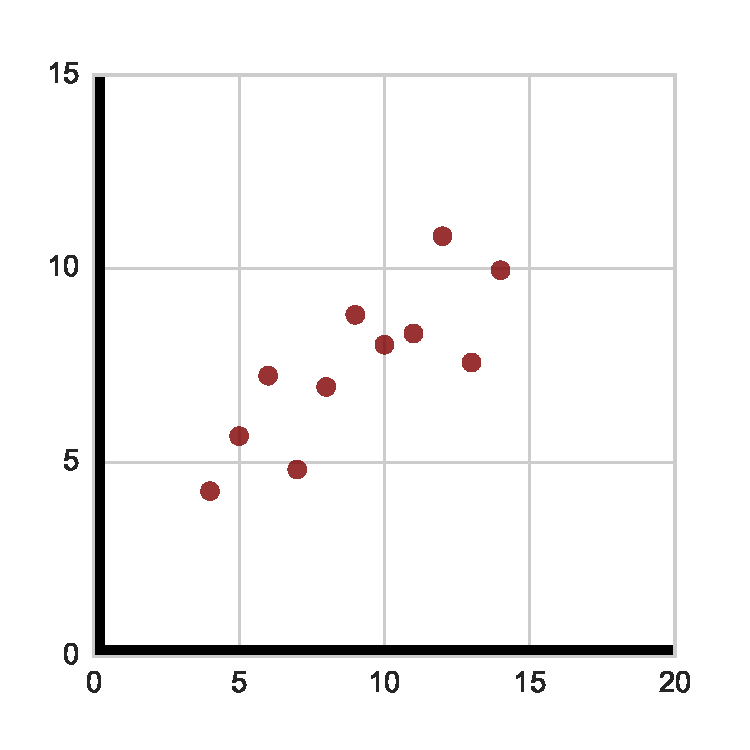
\includegraphics[width=2.7cm]{../anscombeI.pdf} 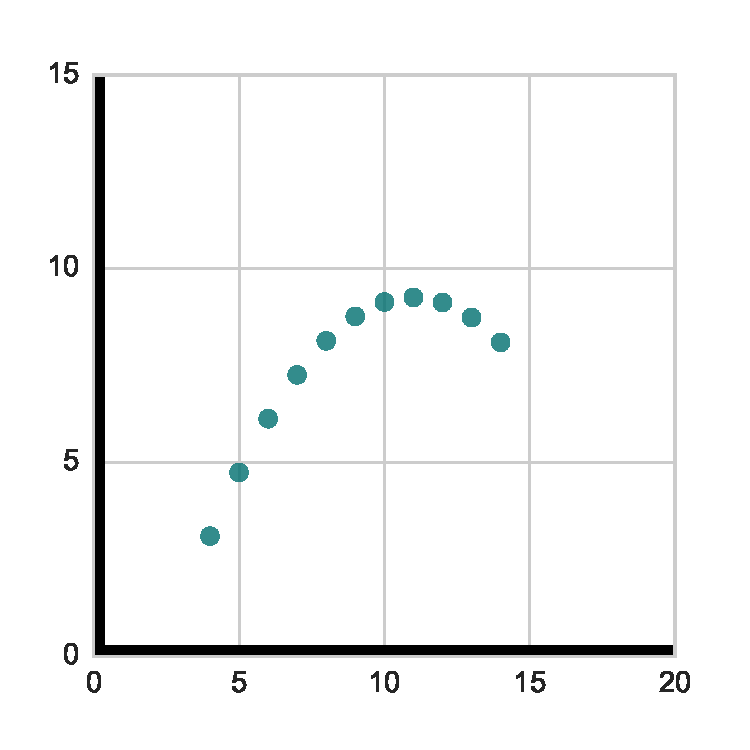
\includegraphics[width=2.7cm]{../anscombeII.pdf} 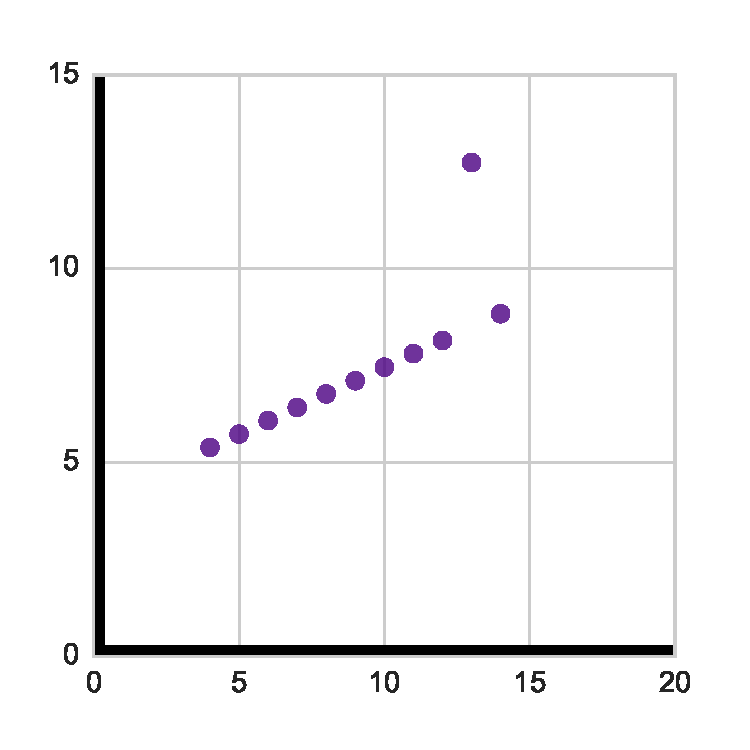
\includegraphics[width=2.7cm]{../anscombeIII.pdf} 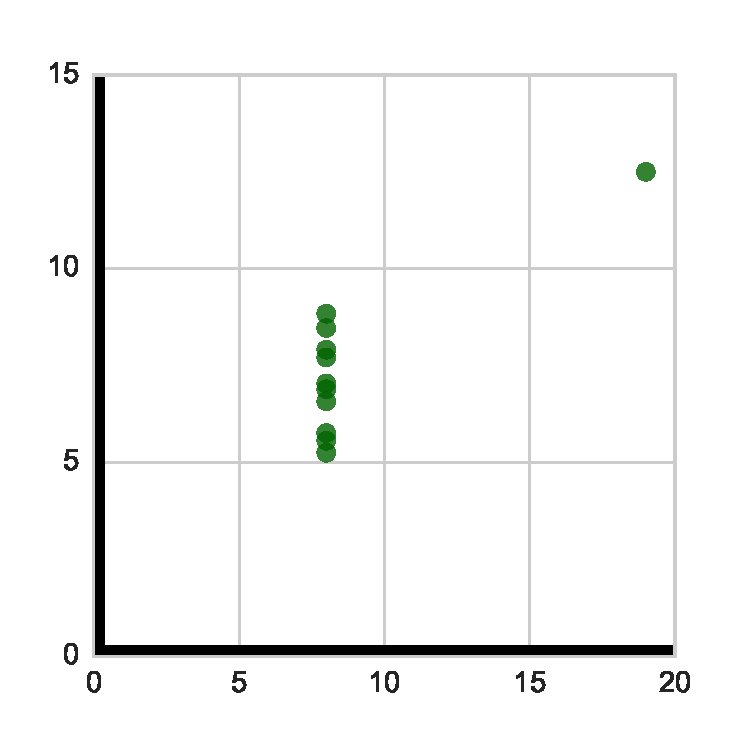
\includegraphics[width=2.7cm]{../anscombeIV.pdf}}



\begin{document}

\frame{\titlepage}

\begin{frame}
\frametitle{Types of Data}
\begin{columns}
\begin{column}{0.5\textwidth}
\begin{center}
\includestandalone[width=0.9\textwidth]{nominal}\\
\includestandalone[width=0.9\textwidth]{quantitative}
\end{center}
\end{column}
\begin{column}{0.5\textwidth}
\begin{center}
\includestandalone[width=0.9\textwidth]{ordinal}\\
\includestandalone[width=0.9\textwidth]{relational}
\end{center}
\end{column}
\end{columns}
\end{frame}

\begin{frame}
\frametitle{Perceptual Accuracy}
\begin{center}
\includestandalone[width=\textwidth]{perceptualaccuracy}
% \vspace{2cm}
\textcolor{orange}{\small{\href{https://youtu.be/k_lvjRCOpJk?list=PLpX1jXuNTXGrjl6CxJ6Cly1GKO1su9yeD}{YouTube: Design Principles in Information Visualisation\newline (Prof. Jessie Kennedy)}}}
\end{center}
\end{frame}


\begin{frame}
\frametitle{\texttt{import matplotlib.pyplot as plt}}
\begin{center}
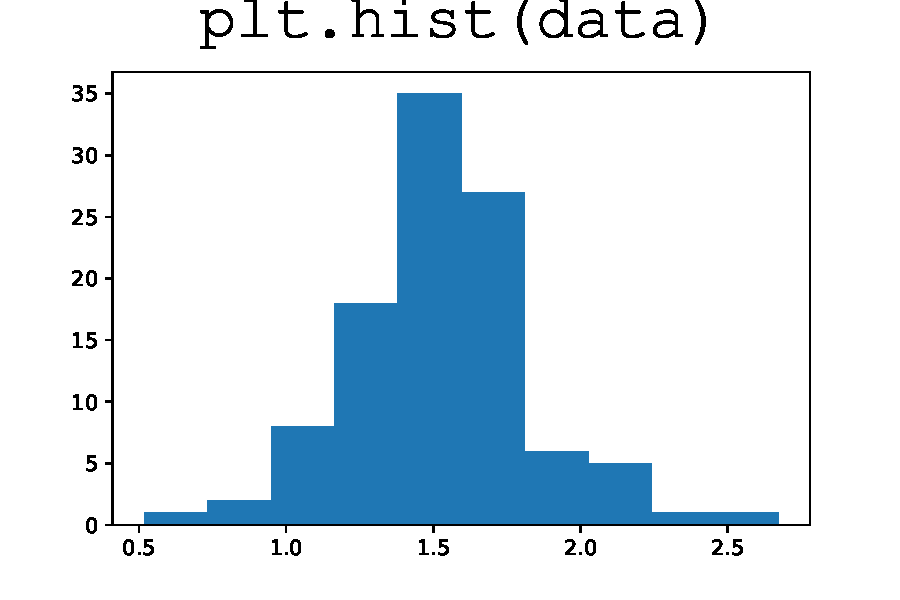
\includegraphics[width=0.33\textwidth]{../hist.pdf}
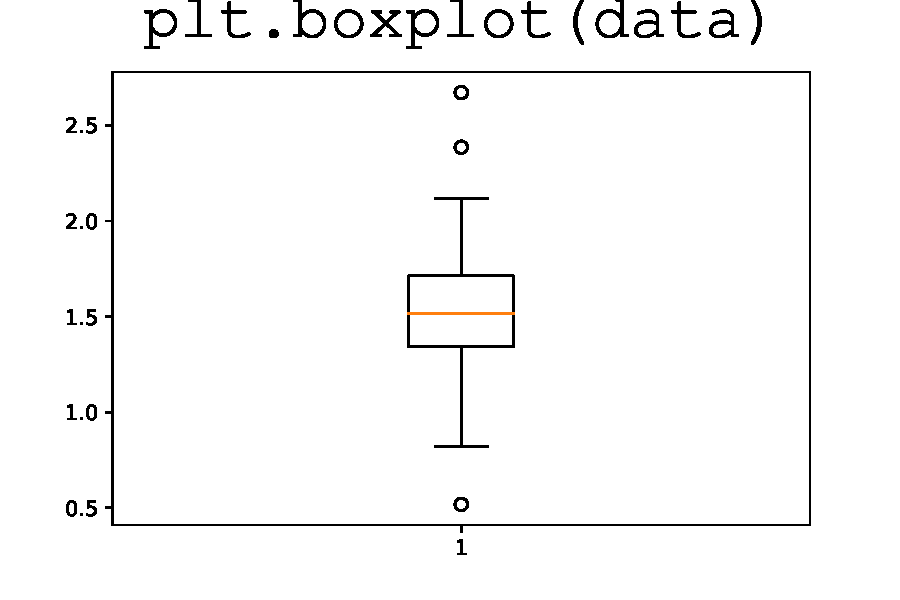
\includegraphics[width=0.33\textwidth]{../box.pdf}
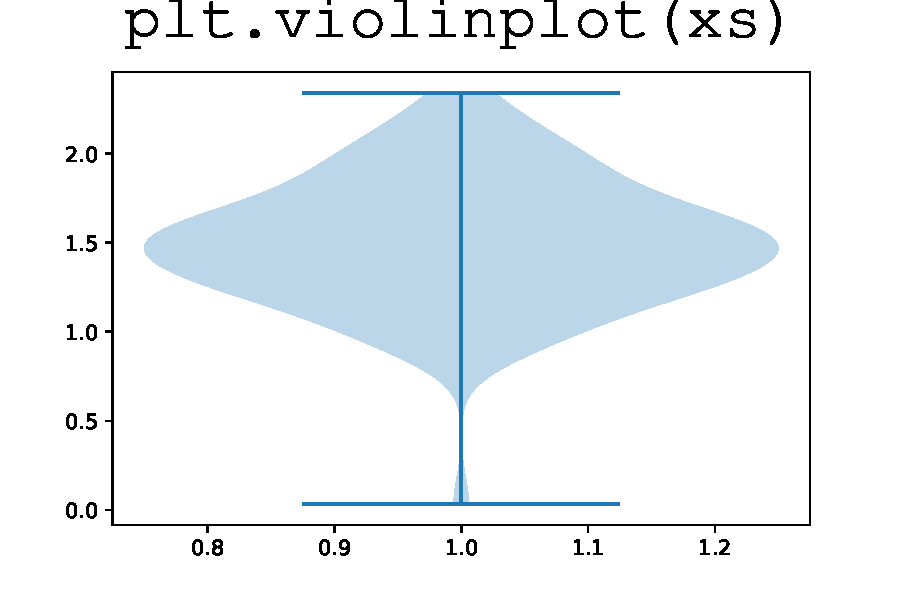
\includegraphics[width=0.33\textwidth]{../violin.pdf}\newline
\vspace{7mm}
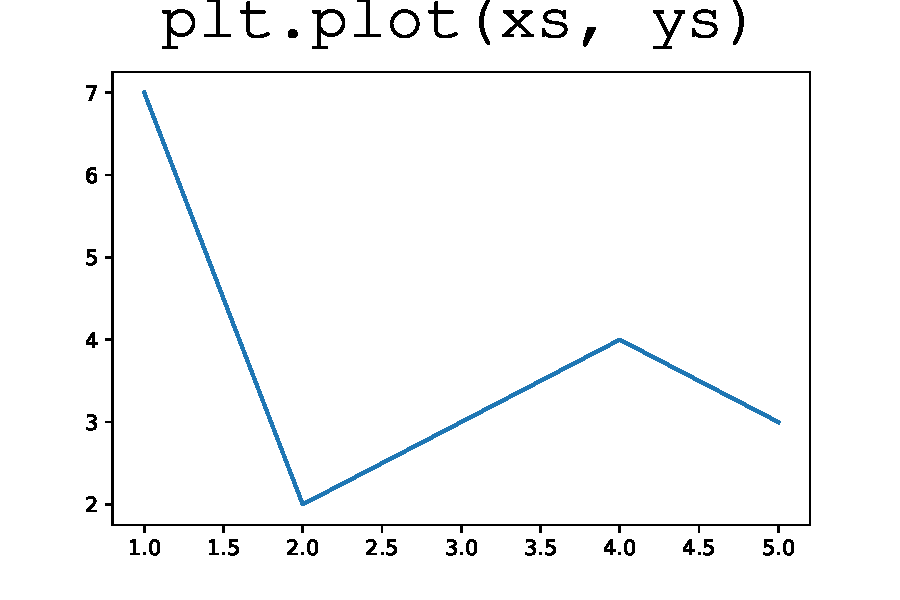
\includegraphics[width=0.33\textwidth]{../line.pdf}
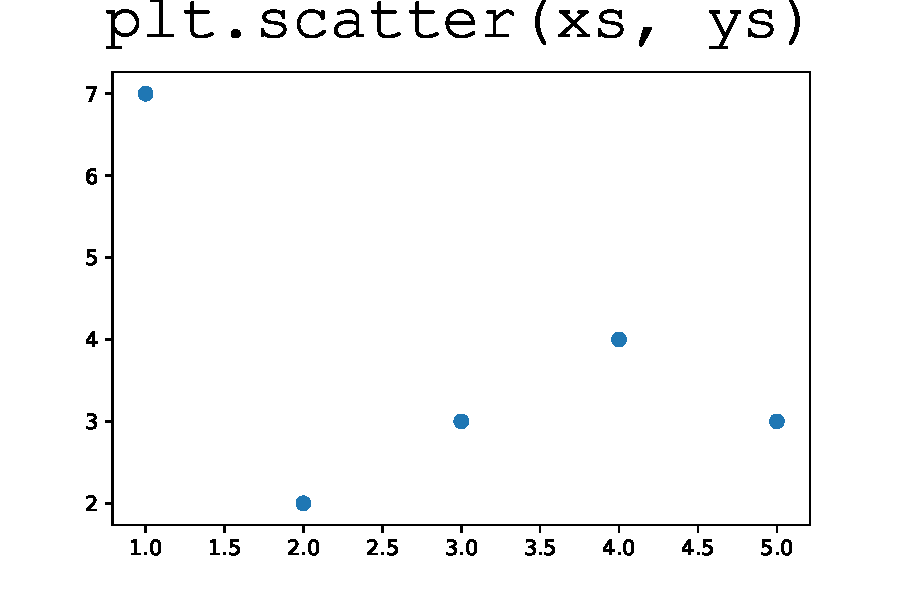
\includegraphics[width=0.33\textwidth]{../scatter.pdf}
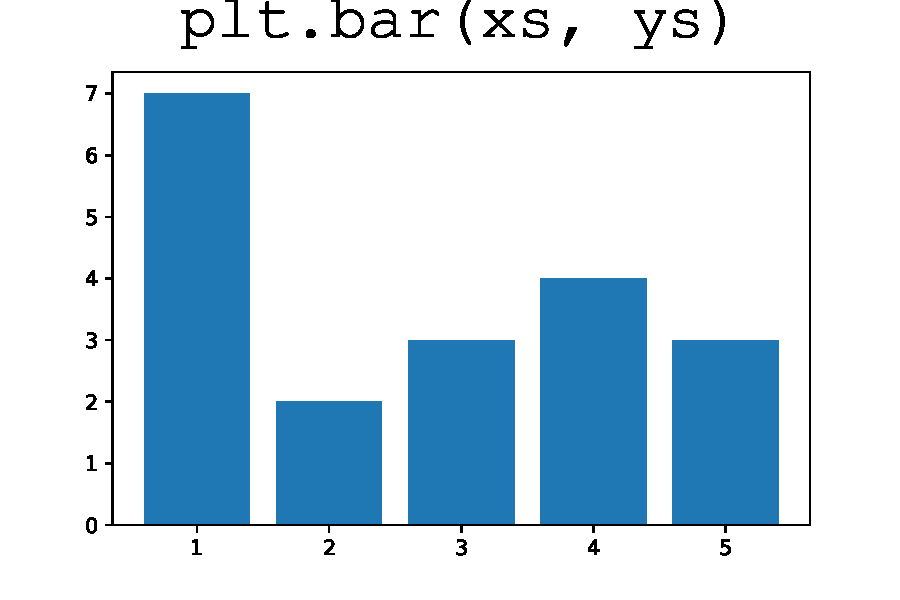
\includegraphics[width=0.33\textwidth]{../bar.pdf}
\end{center}
\end{frame}


\begin{frame}
\frametitle{Anatomy of a Plot}
\includestandalone[width=\textwidth]{anatomy}
\end{frame}

\begin{frame}
\frametitle{Anatomy of a Plot}
\includestandalone[width=\textwidth]{subplots}
\end{frame}

\begin{frame}[fragile]
\frametitle{Women's 200m Olympic Medallists}
\footnotesize{
\begin{center}
\begin{tabular}{clccc}
\toprule
Year & Athlete & Medal & Country & Result \\
\midrule
1948 & Fanny Blankers-Koen & GOLD & NED & 24.40 \\
1948 & Audrey Williamson & SILVER & GBR & 25.10 \\
1948 & Audrey Patterson & BRONZE & USA & 25.20 \\
1952 & Marjorie Jackson & GOLD & AUS & 23.70 \\
1952 & Bertha Brouwer & SILVER & NED & 24.20 \\
$\vdots$ & $\vdots$ & $\vdots$ & $\vdots$ & $\vdots$ \\
2008 & Allyson Felix & SILVER & USA & 21.93 \\
2008 & Kerron Stewart & BRONZE & JAM & 22.00 \\
\bottomrule
\end{tabular}
\end{center}
}
\end{frame}


\begin{frame}[fragile]
\tiny{
\begin{columns}
\begin{column}{0.45\textwidth}
\begin{minted}{python}
fig, ax = plt.subplots(1)

ax.plot(dates, gold)

ax.plot(dates, silver)

ax.plot(dates, bronze)
















plt.show()
\end{minted}
\end{column}
\begin{column}{0.55\textwidth}
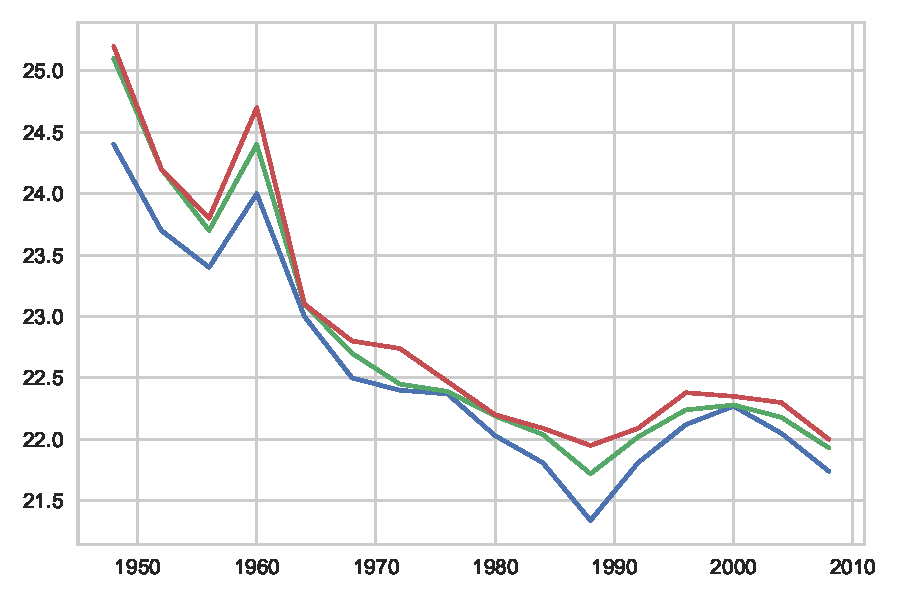
\includegraphics[width=\textwidth]{../olympics_1.pdf}
\end{column}
\end{columns}
}
\end{frame}

\begin{frame}[fragile]
\tiny{
\begin{columns}
\begin{column}{0.45\textwidth}
\begin{minted}{python}
fig, ax = plt.subplots(1)

ax.plot(dates, gold, c='darkgoldenrod')

ax.plot(dates, silver, c='slategray')

ax.plot(dates, bronze, c='sienna')
















plt.show()
\end{minted}
\end{column}
\begin{column}{0.55\textwidth}
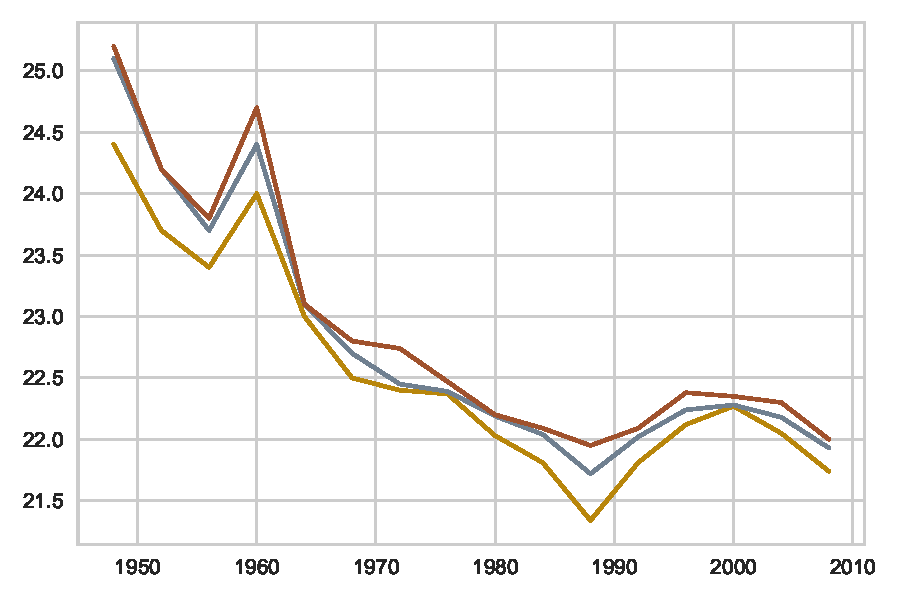
\includegraphics[width=\textwidth]{../olympics_2.pdf}
\end{column}
\end{columns}
}
\end{frame}

\begin{frame}[fragile]
\tiny{
\begin{columns}
\begin{column}{0.45\textwidth}
\begin{minted}{python}
fig, ax = plt.subplots(1)

ax.plot(dates, gold, c='darkgoldenrod')

ax.plot(dates, silver, c='slategray')

ax.plot(dates, bronze, c='sienna')









ax.set_xticks(dates)
ax.set_xticklabels(dates, rotation='vertical')





plt.show()
\end{minted}
\end{column}
\begin{column}{0.55\textwidth}
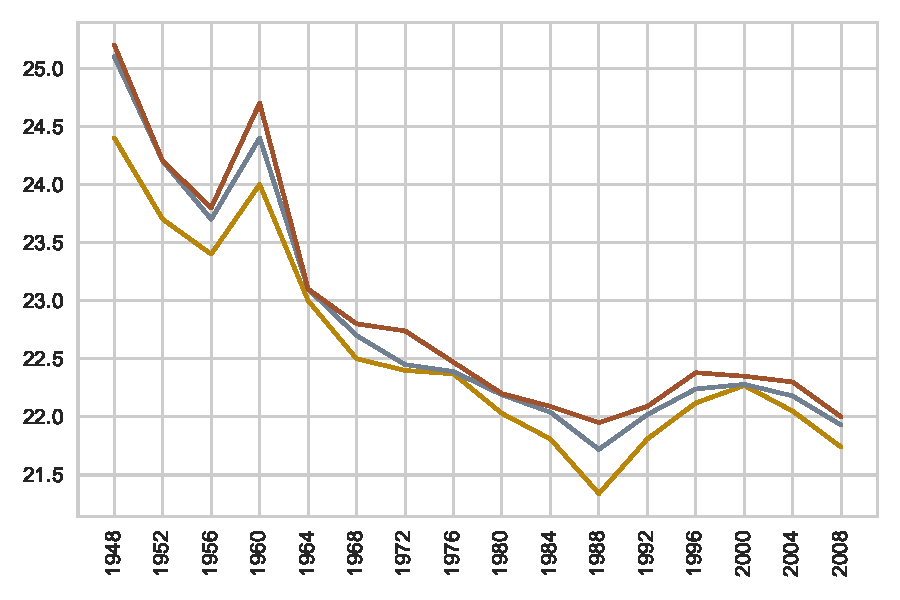
\includegraphics[width=\textwidth]{../olympics_3.pdf}
\end{column}
\end{columns}
}
\end{frame}

\begin{frame}[fragile]
\tiny{
\begin{columns}
\begin{column}{0.45\textwidth}
\begin{minted}{python}
fig, ax = plt.subplots(1)

ax.plot(dates, gold, c='darkgoldenrod')

ax.plot(dates, silver, c='slategray')

ax.plot(dates, bronze, c='sienna')









ax.set_xticks(dates)
ax.set_xticklabels(dates, rotation='vertical')

ax.set_xlabel("Year")
ax.set_ylabel("Time")
ax.set_title("Women's 200m Olympic Medalists", fontsize=18)

plt.show()
\end{minted}
\end{column}
\begin{column}{0.55\textwidth}
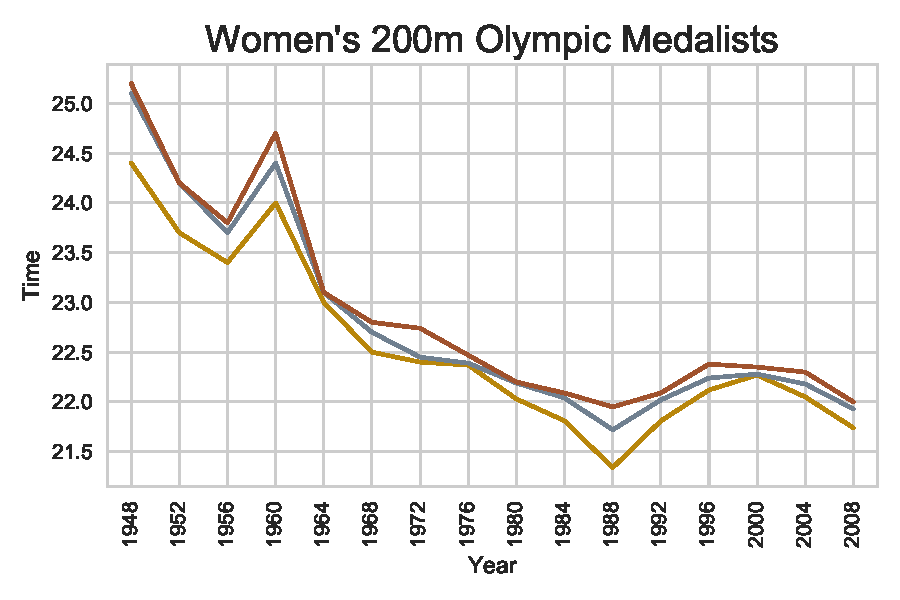
\includegraphics[width=\textwidth]{../olympics_4.pdf}
\end{column}
\end{columns}
}
\end{frame}

\begin{frame}[fragile]
\tiny{
\begin{columns}
\begin{column}{0.45\textwidth}
\begin{minted}{python}
fig, ax = plt.subplots(1)

ax.plot(dates, gold, c='darkgoldenrod')

ax.plot(dates, silver, c='slategray')

ax.plot(dates, bronze, c='sienna')


ax.scatter(usa_x, usa_y, lw=0.8,
           facecolor='black',
           marker='*', s=100)




ax.set_xticks(dates)
ax.set_xticklabels(dates, rotation='vertical')

ax.set_xlabel("Year")
ax.set_ylabel("Time")
ax.set_title("Women's 200m Olympic Medalists", fontsize=18)

plt.show()
\end{minted}
\end{column}
\begin{column}{0.55\textwidth}
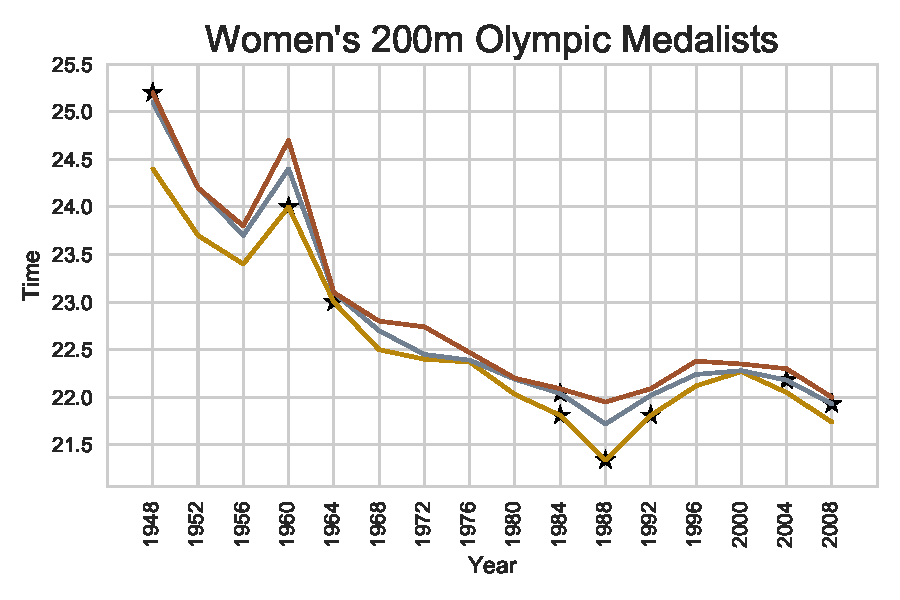
\includegraphics[width=\textwidth]{../olympics_5.pdf}
\end{column}
\end{columns}
}
\end{frame}


\begin{frame}[fragile]
\tiny{
\begin{columns}
\begin{column}{0.45\textwidth}
\begin{minted}{python}
fig, ax = plt.subplots(1)

ax.plot(dates, gold, c='darkgoldenrod',
        zorder=1)
ax.plot(dates, silver, c='slategray',
        zorder=1)
ax.plot(dates, bronze, c='sienna',
        zorder=1)

ax.scatter(usa_x, usa_y, lw=0.8,
           facecolor='black',
           marker='*', s=100,
           zorder=2)



ax.set_xticks(dates)
ax.set_xticklabels(dates, rotation='vertical')

ax.set_xlabel("Year")
ax.set_ylabel("Time")
ax.set_title("Women's 200m Olympic Medalists", fontsize=18)

plt.show()
\end{minted}
\end{column}
\begin{column}{0.55\textwidth}
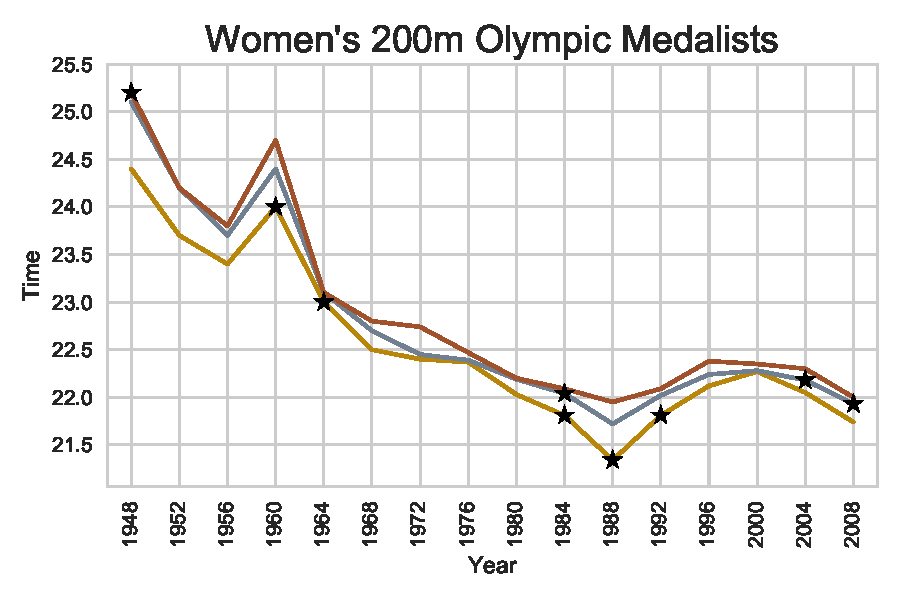
\includegraphics[width=\textwidth]{../olympics_6.pdf}
\end{column}
\end{columns}
}
\end{frame}

\begin{frame}[fragile]
\tiny{
\begin{columns}
\begin{column}{0.45\textwidth}
\begin{minted}{python}
fig, ax = plt.subplots(1)

ax.plot(dates, gold, c='darkgoldenrod',
        zorder=1)
ax.plot(dates, silver, c='slategray',
        zorder=1)
ax.plot(dates, bronze, c='sienna',
        zorder=1)

ax.scatter(usa_x, usa_y, lw=0.8,
           facecolor='black',
           marker='*', s=100,
           zorder=2)

plt.legend()

ax.set_xticks(dates)
ax.set_xticklabels(dates, rotation='vertical')

ax.set_xlabel("Year")
ax.set_ylabel("Time")
ax.set_title("Women's 200m Olympic Medalists", fontsize=18)

plt.show()
\end{minted}
\end{column}
\begin{column}{0.55\textwidth}
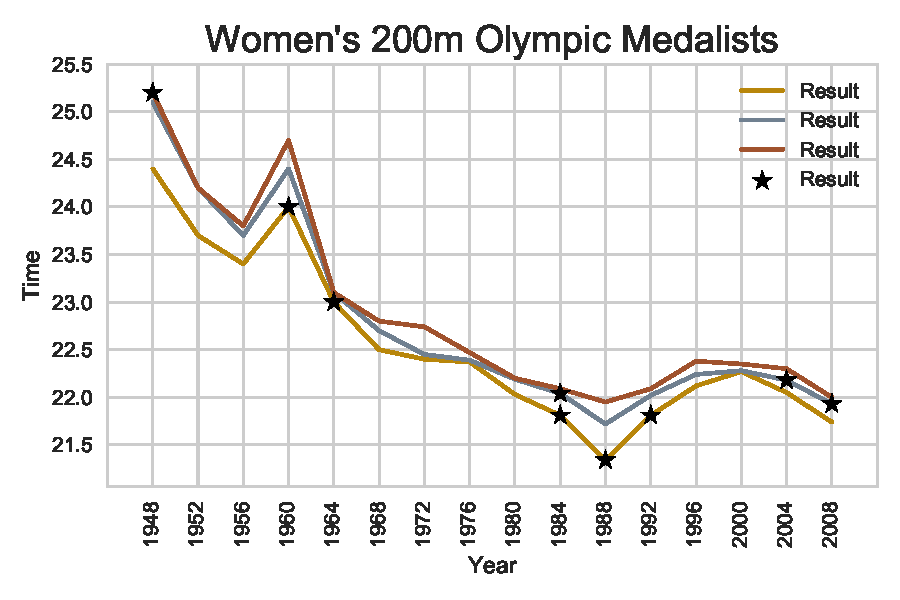
\includegraphics[width=\textwidth]{../olympics_7.pdf}
\end{column}
\end{columns}
}
\end{frame}


\begin{frame}[fragile]
\tiny{
\begin{columns}
\begin{column}{0.45\textwidth}
\begin{minted}{python}
fig, ax = plt.subplots(1)

ax.plot(dates, gold, c='darkgoldenrod',
        zorder=1, label='Gold Medal')
ax.plot(dates, silver, c='slategray',
        zorder=1, label='Silver Medal')
ax.plot(dates, bronze, c='sienna',
        zorder=1, label='Bronze Medal')

ax.scatter(usa_x, usa_y, lw=0.8,
           facecolor='black',
           marker='*', s=100,
           zorder=2, label='USA Athletes')

plt.legend()

ax.set_xticks(dates)
ax.set_xticklabels(dates, rotation='vertical')

ax.set_xlabel("Year")
ax.set_ylabel("Time")
ax.set_title("Women's 200m Olympic Medalists", fontsize=18)

plt.show()
\end{minted}
\end{column}
\begin{column}{0.55\textwidth}
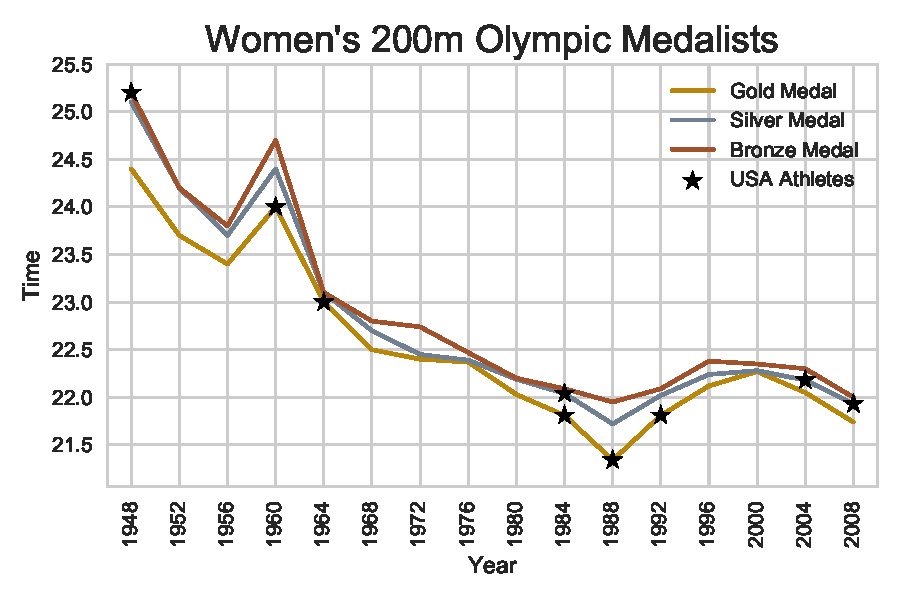
\includegraphics[width=\textwidth]{../olympics_8.pdf}
\end{column}
\end{columns}
}
\end{frame}

\begin{frame}
\frametitle{Choosing Colormaps}
\begin{center}
\textcolor{orange}{
\href{https://www.youtube.com/watch?v=xAoljeRJ3lU}{YouTube: A Better Default Colormap for Matplotlib -\newline SciPy 2015 (Nathaniel Smith and Stéfan van der Walt)}
}
\end{center}
\end{frame}

\begin{frame}
\begin{figure}
    % \frametitle{Choosing Colormaps}
    \begin{columns}
	\begin{column}{0.45\textwidth}
		\begin{center}
		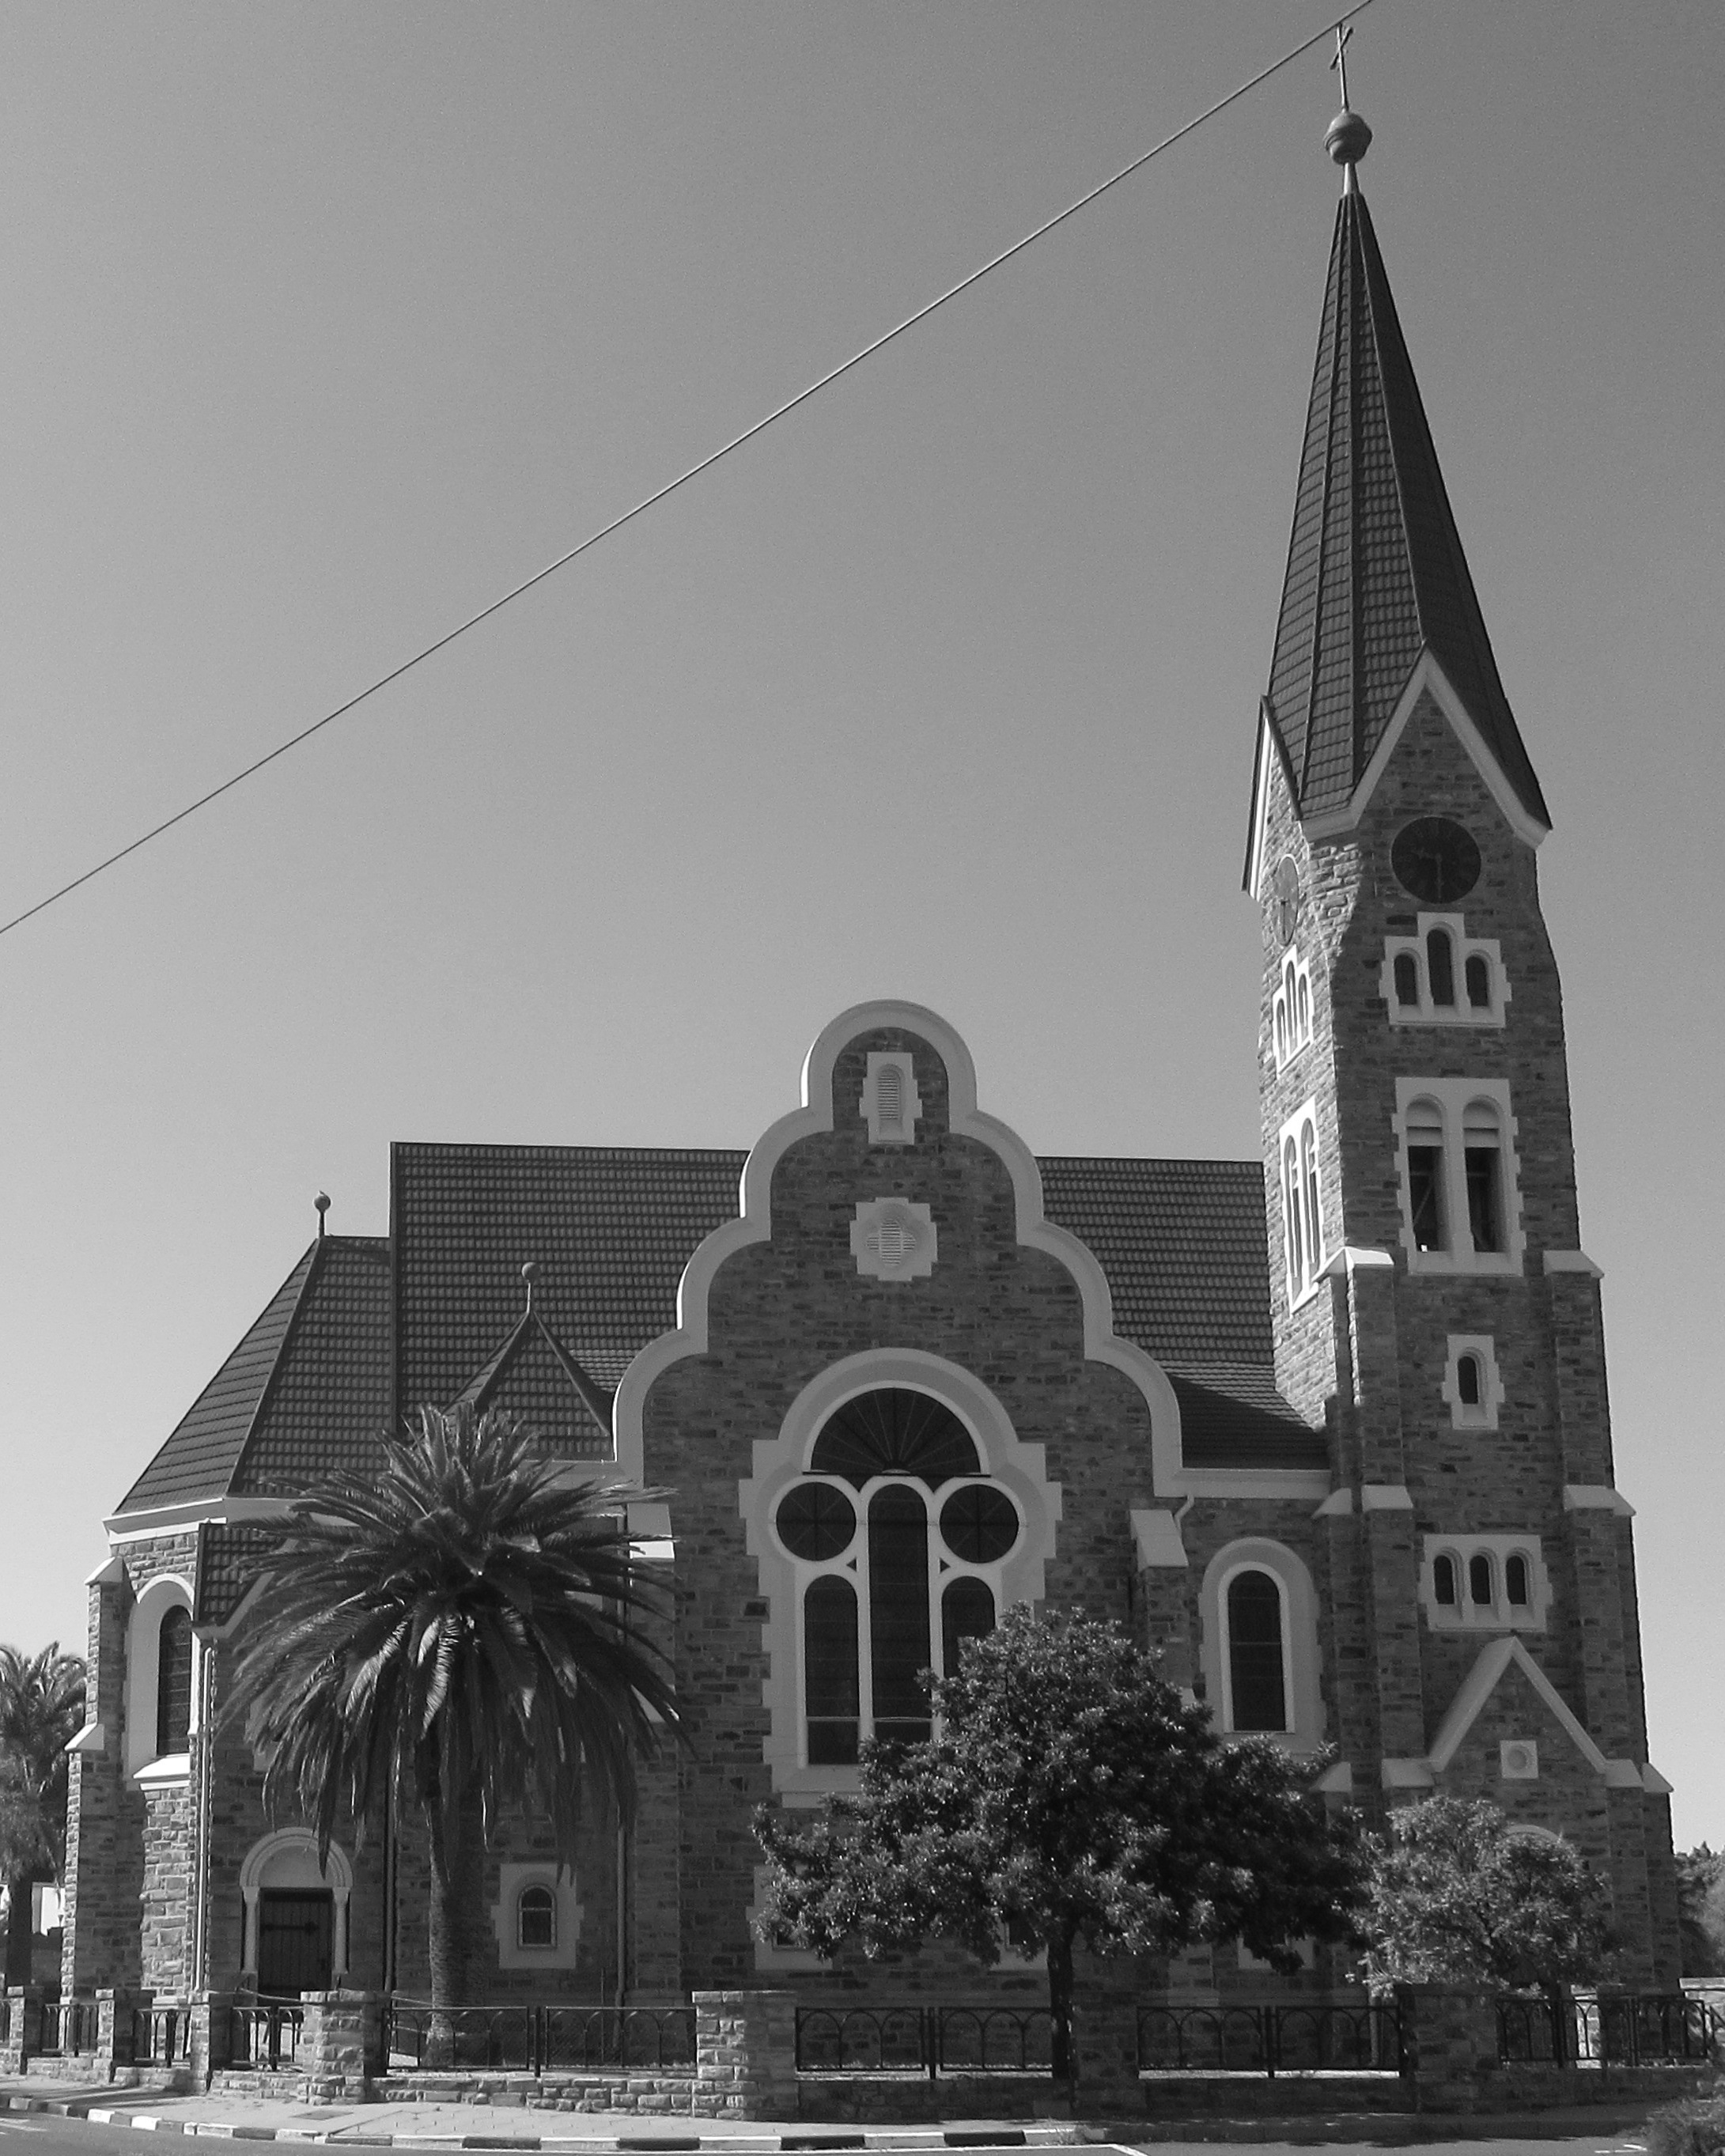
\includegraphics[width=0.9\textwidth]{../testimage.jpg}
		\end{center}
	\end{column}
	\begin{column}{0.55\textwidth}
		\scriptsize{
		\begin{equation*}
		\begin{pmatrix}
		47 & 58 & 69 & 80 & 1 & 12 & 23 & 34 & 45 \\
    	57 & 68 & 79 & 9 & 11 & 22 & 33 & 44 & 46 \\
    	67 & 78 & 8 & 10 & 21 & 32 & 43 & 54 & 56 \\
    	77 & 7 & 18 & 20 & 31 & 42 & 53 & 55 & 66 \\
    	6 & 17 & 19 & 30 & 41 & 52 & 63 & 65 & 76 \\
    	16 & 27 & 29 & 40 & 51 & 62 & 64 & 75 & 5 \\
    	26 & 28 & 39 & 50 & 61 & 72 & 74 & 4 & 15 \\
    	36 & 38 & 49 & 60 & 71 & 73 & 3 & 14 & 25 \\
    	37 & 48 & 59 & 70 & 81 & 2 & 13 & 24 & 35
		\end{pmatrix}
		\end{equation*}
		}
	\end{column}
	\end{columns}
\end{figure}
\end{frame}

\begin{frame}
\begin{center}
\semitransp[0]{Perceptually Uniform Sequencial Colormaps}
\end{center}
\begin{columns}
\begin{column}{0.5\textwidth}
\begin{center}
\vfill
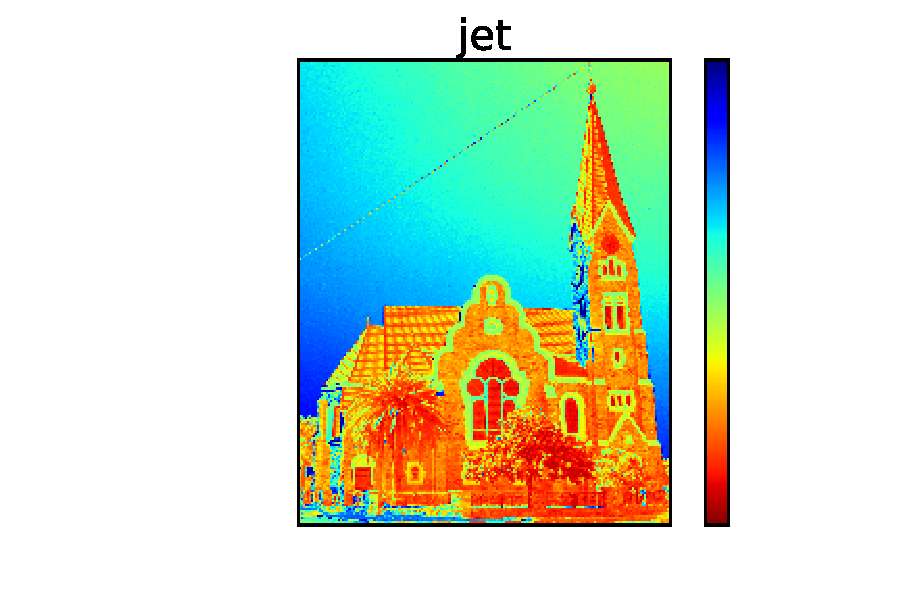
\includegraphics[width=0.42\textwidth]{../church_jet.pdf}
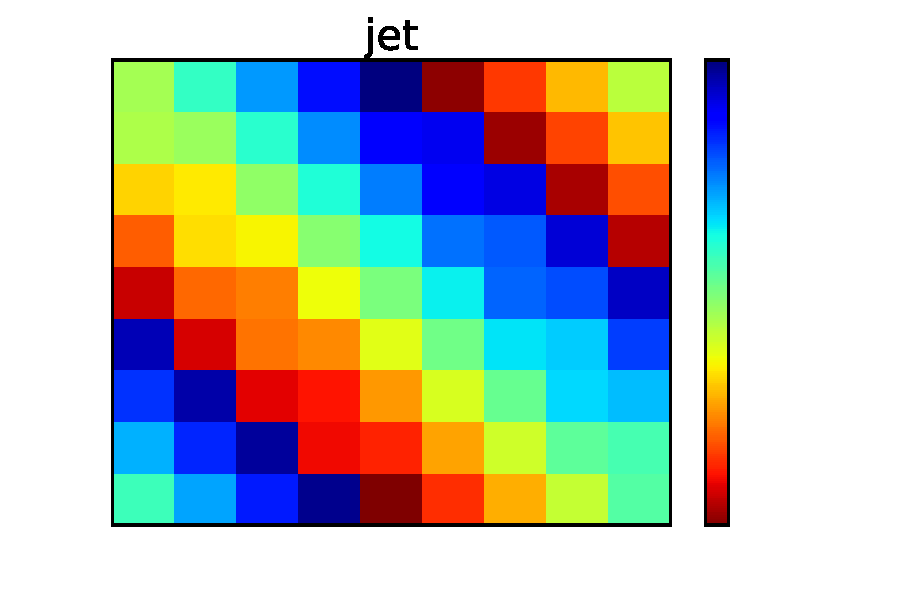
\includegraphics[width=0.58\textwidth]{../magicsquare_jet.pdf}\newline\newline
\vfill
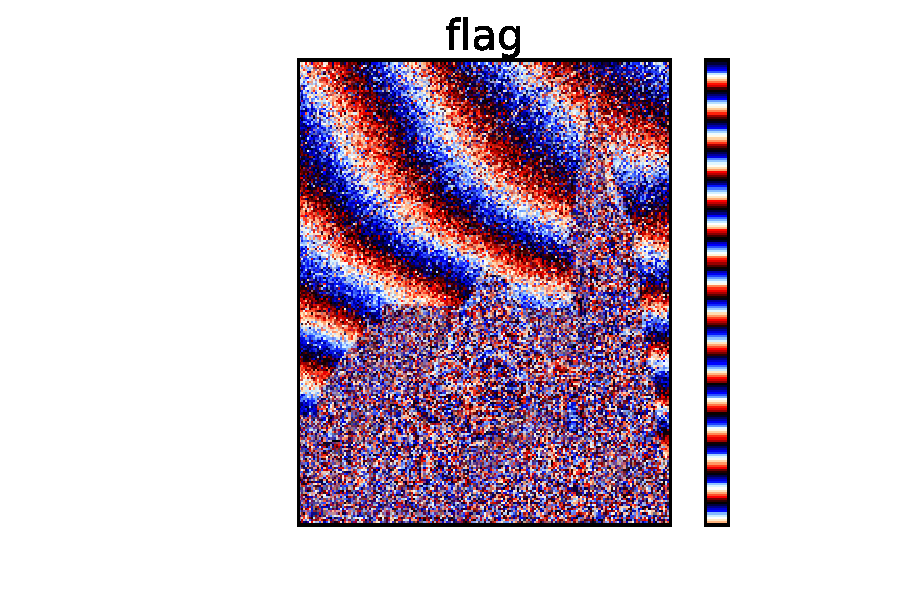
\includegraphics[width=0.42\textwidth]{../church_flag.pdf}
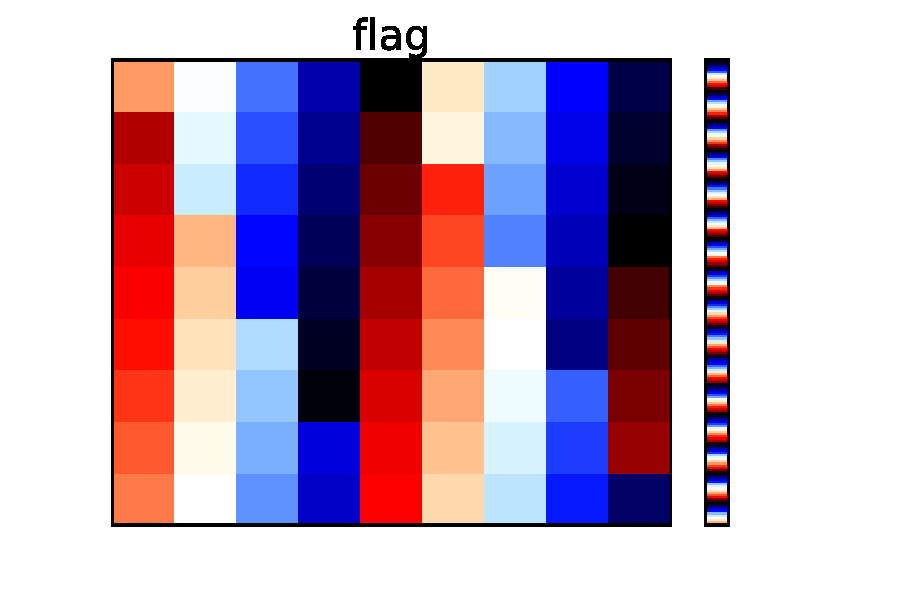
\includegraphics[width=0.58\textwidth]{../magicsquare_flag.pdf}
\vfill
\end{center}
\end{column}
\begin{column}{0.5\textwidth}
\begin{center}
\vfill
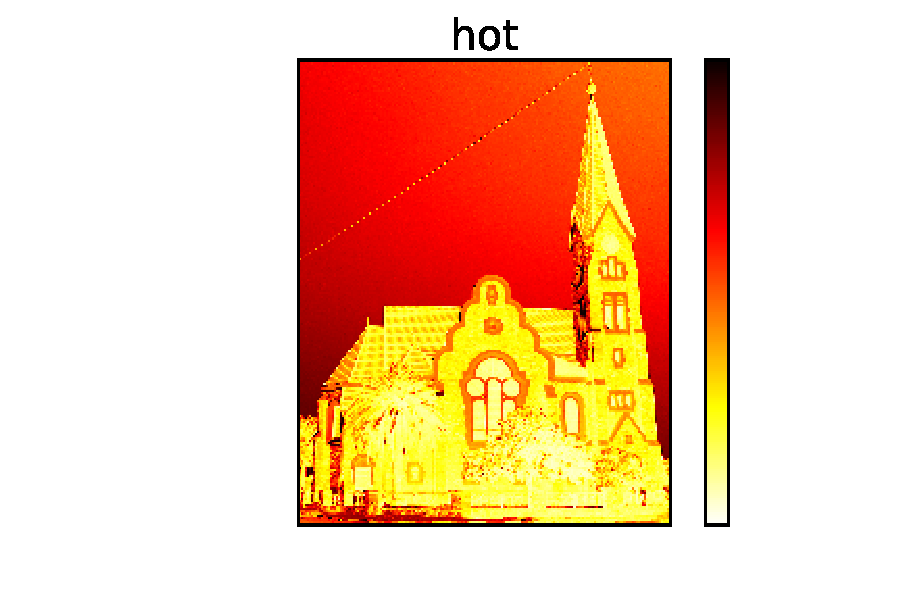
\includegraphics[width=0.42\textwidth]{../church_hot.pdf}
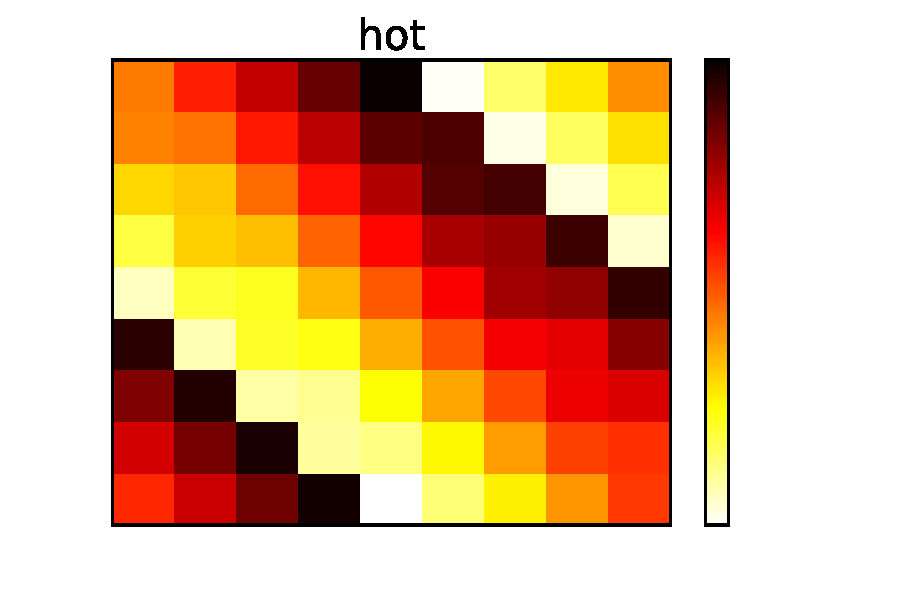
\includegraphics[width=0.58\textwidth]{../magicsquare_hot.pdf}\newline\newline
\vfill
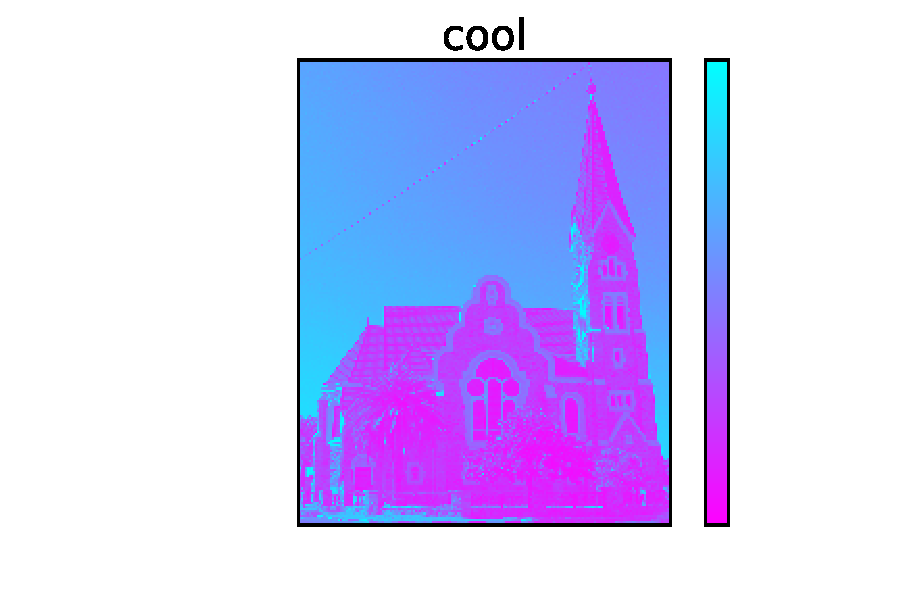
\includegraphics[width=0.42\textwidth]{../church_cool.pdf}
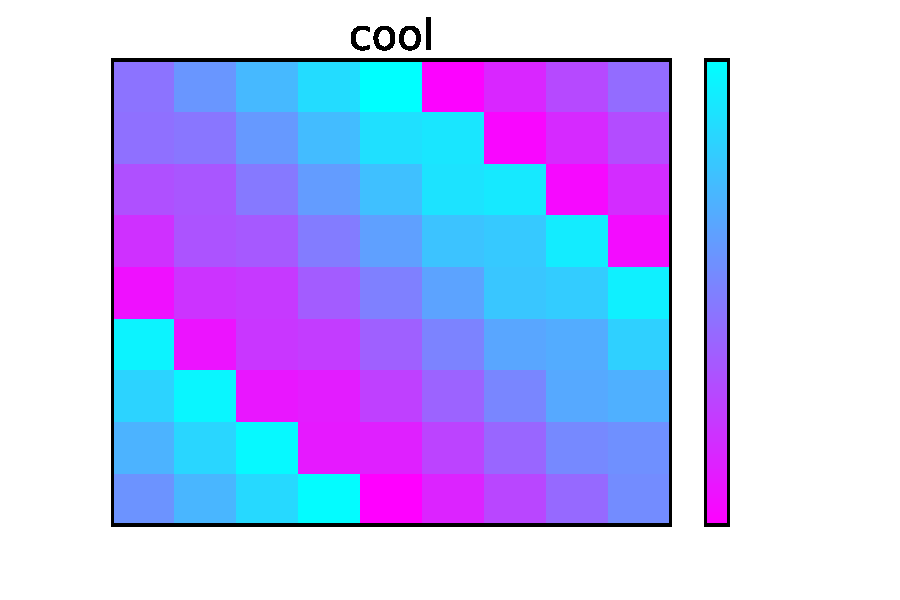
\includegraphics[width=0.58\textwidth]{../magicsquare_cool.pdf}
\vfill
\end{center}
\end{column}
\end{columns}
\end{frame}

\begin{frame}
\begin{center}
\semitransp[0]{Perceptually Uniform Sequencial Colormaps}
\end{center}
\begin{columns}
\begin{column}{0.5\textwidth}
\begin{center}
\vfill
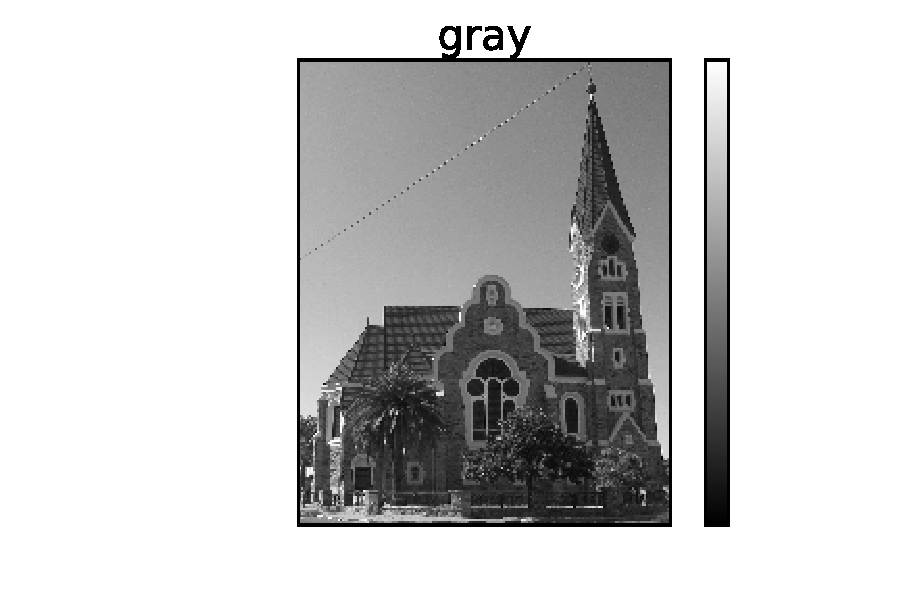
\includegraphics[width=0.42\textwidth]{../church_gray.pdf}
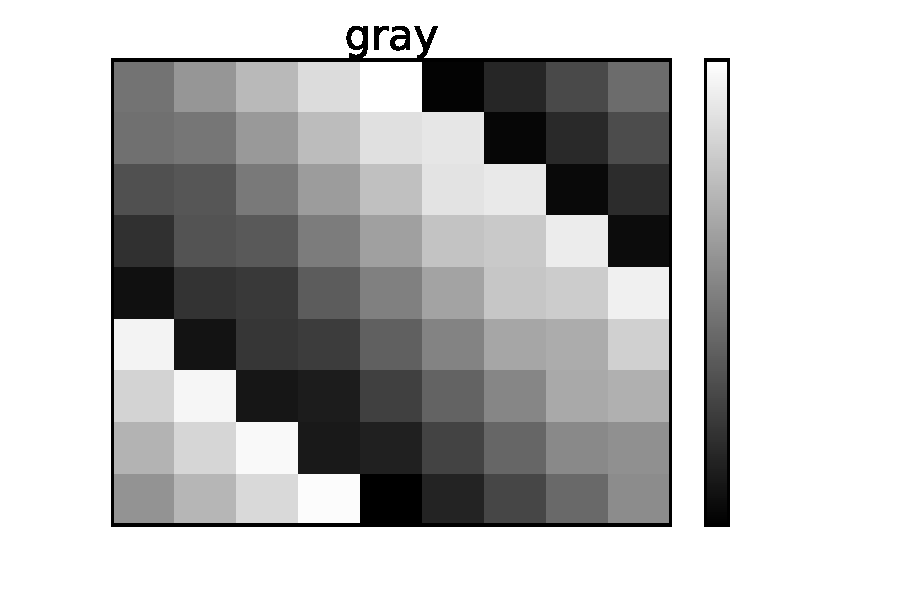
\includegraphics[width=0.58\textwidth]{../magicsquare_gray.pdf}\newline\newline
\vfill
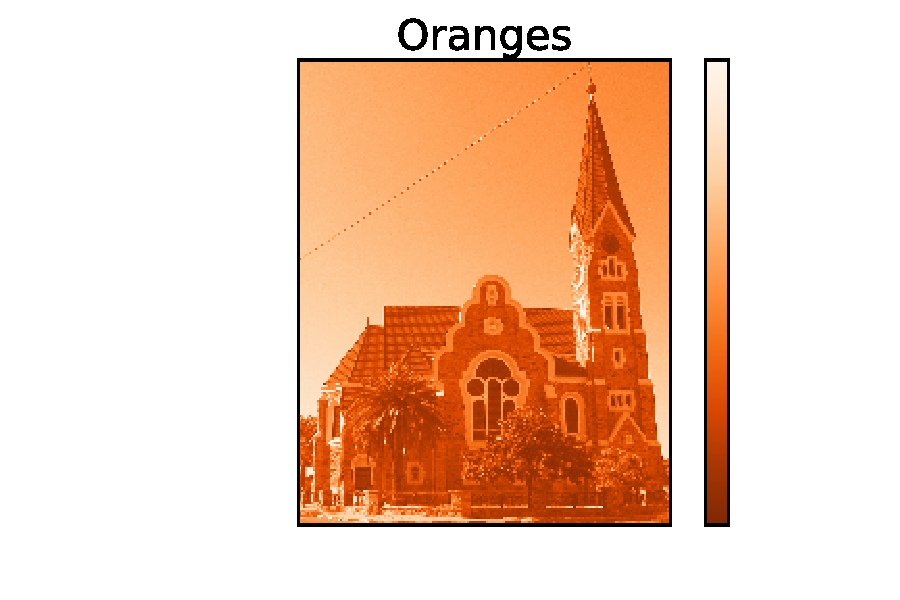
\includegraphics[width=0.42\textwidth]{../church_Oranges.pdf}
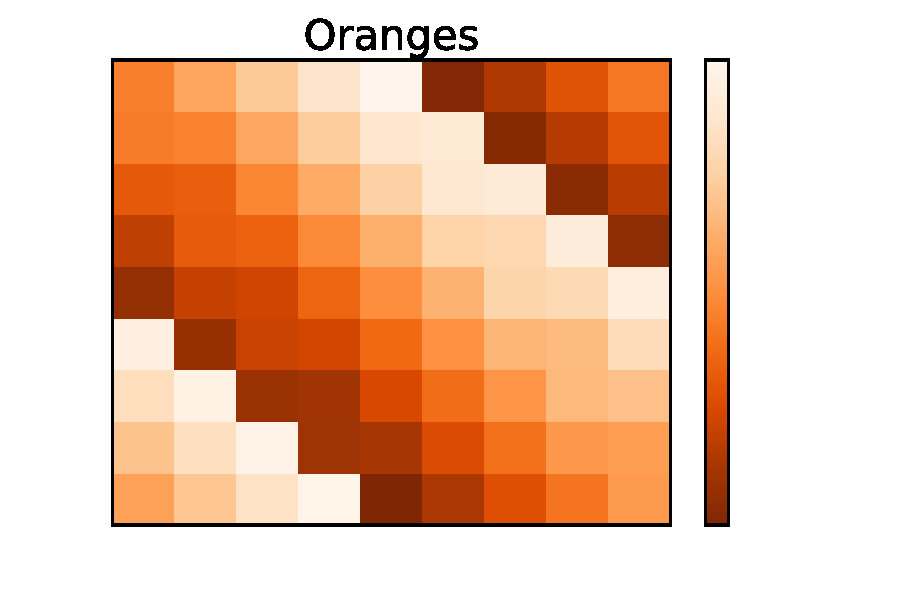
\includegraphics[width=0.58\textwidth]{../magicsquare_Oranges.pdf}
\vfill
\end{center}
\end{column}
\begin{column}{0.5\textwidth}
\begin{center}
\vfill
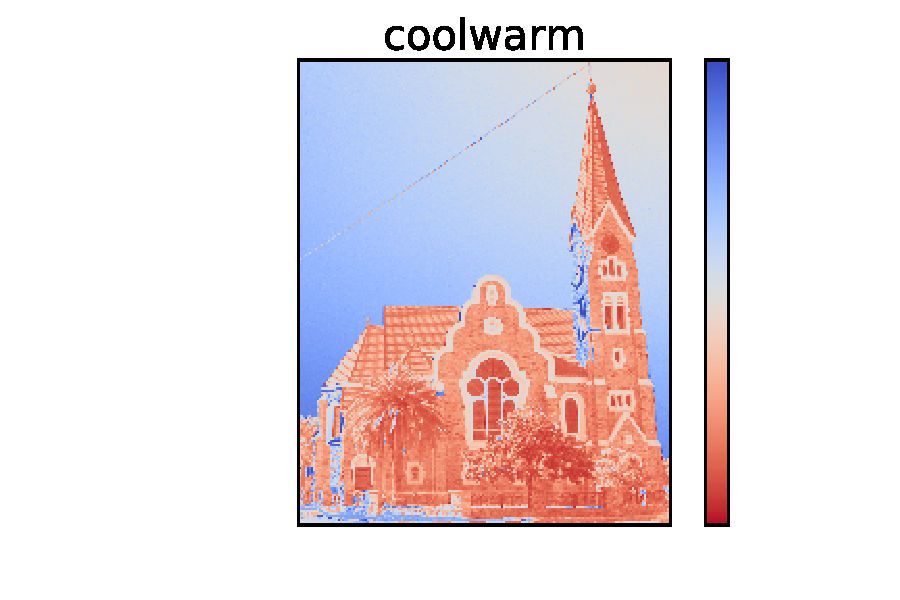
\includegraphics[width=0.42\textwidth]{../church_coolwarm.pdf}
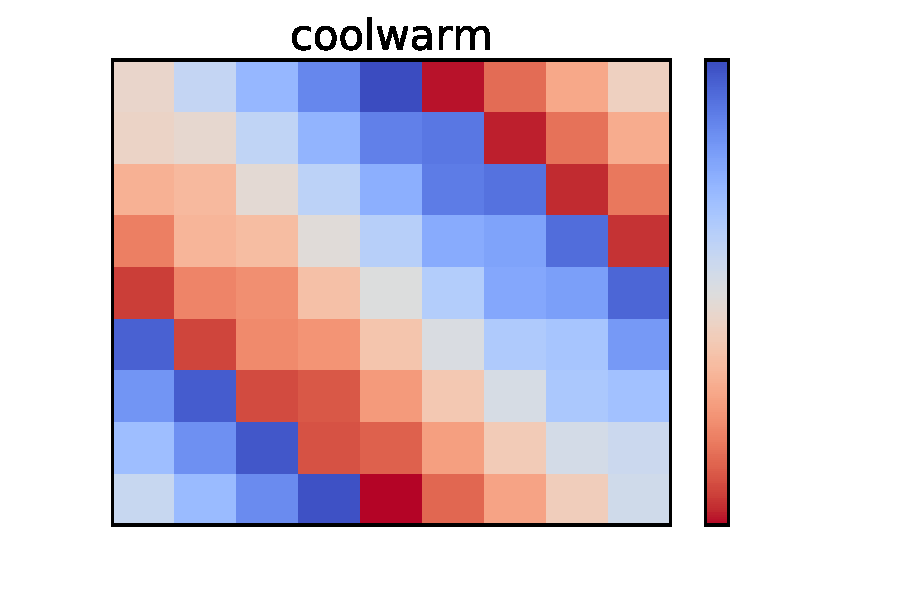
\includegraphics[width=0.58\textwidth]{../magicsquare_coolwarm.pdf}\newline\newline
\vfill
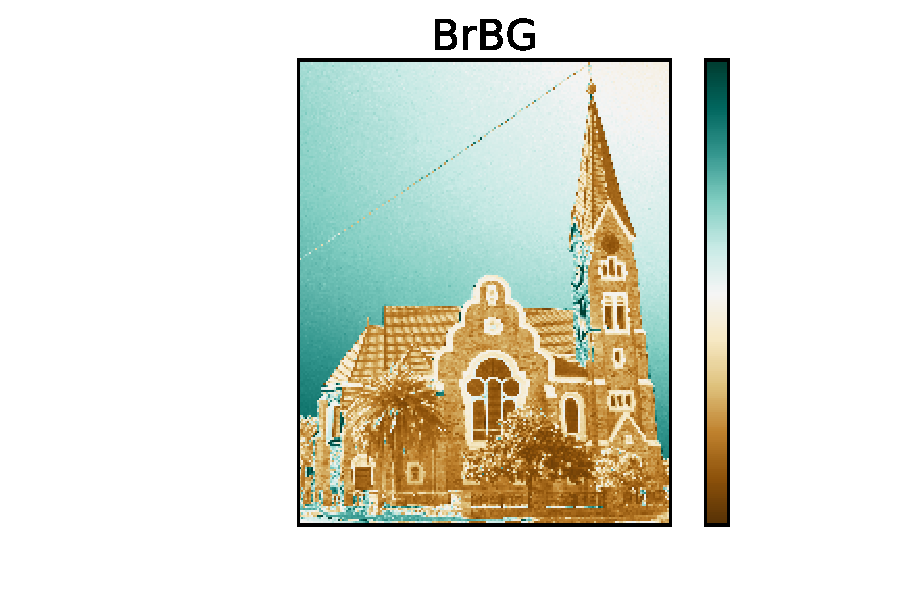
\includegraphics[width=0.42\textwidth]{../church_BrBG.pdf}
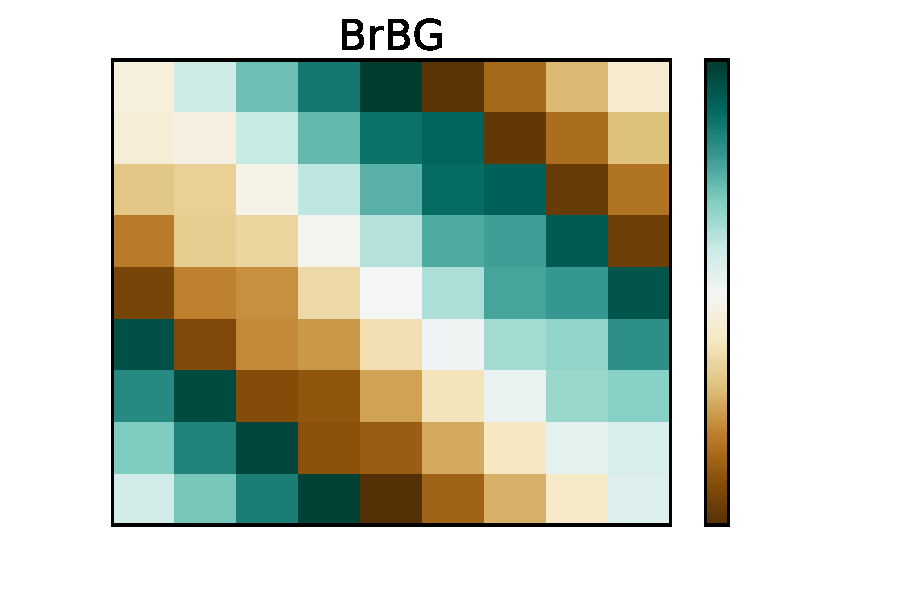
\includegraphics[width=0.58\textwidth]{../magicsquare_BrBG.pdf}
\vfill
\end{center}
\end{column}
\end{columns}
\end{frame}

\begin{frame}
\begin{center}
\textit{Perceptually Uniform Sequencial Colormaps}
\end{center}
\begin{columns}
\begin{column}{0.5\textwidth}
\begin{center}
\vfill
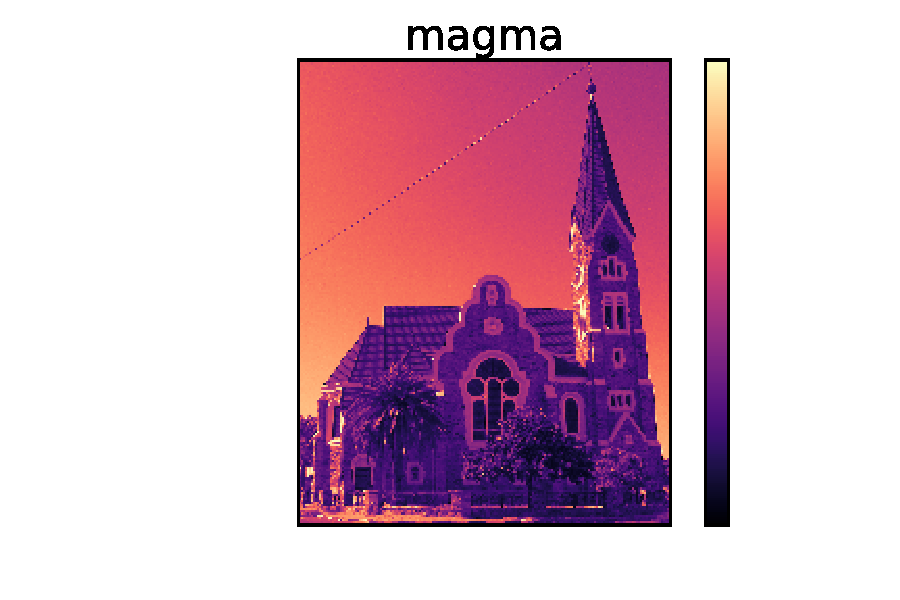
\includegraphics[width=0.42\textwidth]{../church_magma.pdf}
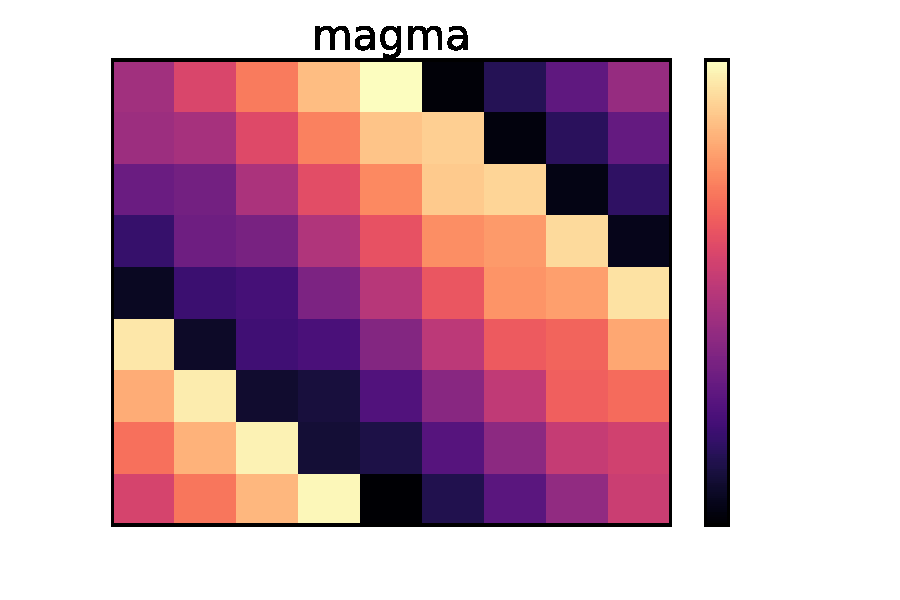
\includegraphics[width=0.58\textwidth]{../magicsquare_magma.pdf}\newline\newline
\vfill
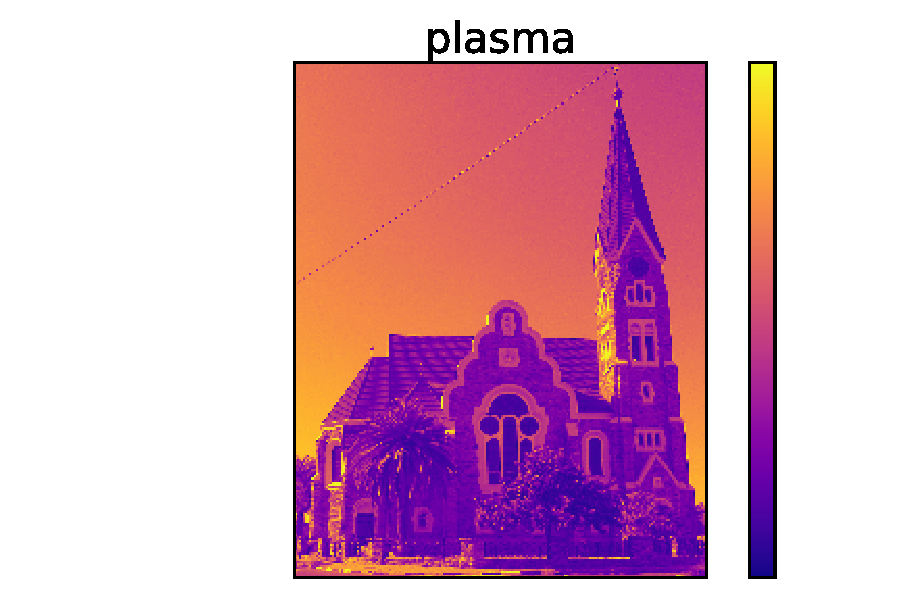
\includegraphics[width=0.42\textwidth]{../church_plasma.pdf}
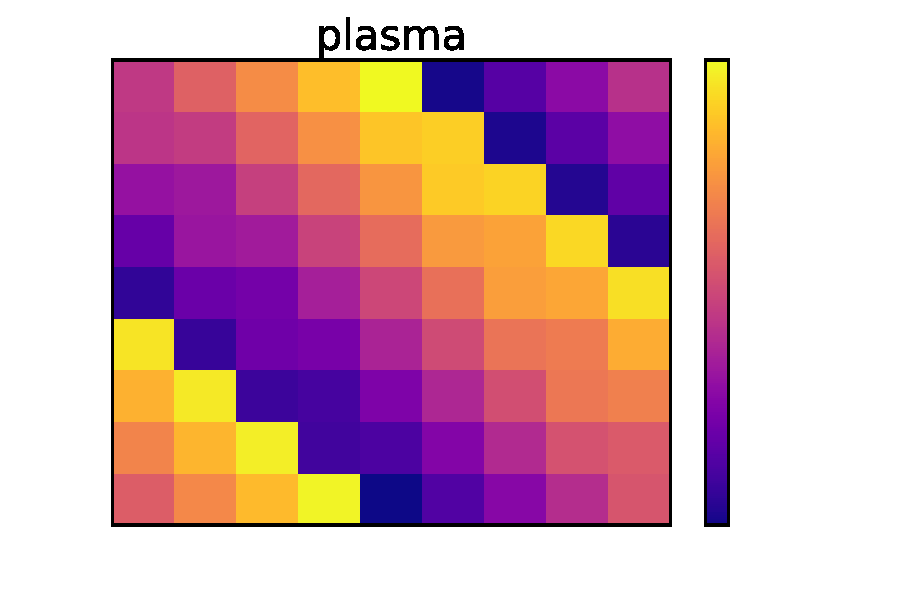
\includegraphics[width=0.58\textwidth]{../magicsquare_plasma.pdf}
\vfill
\end{center}
\end{column}
\begin{column}{0.5\textwidth}
\begin{center}
\vfill
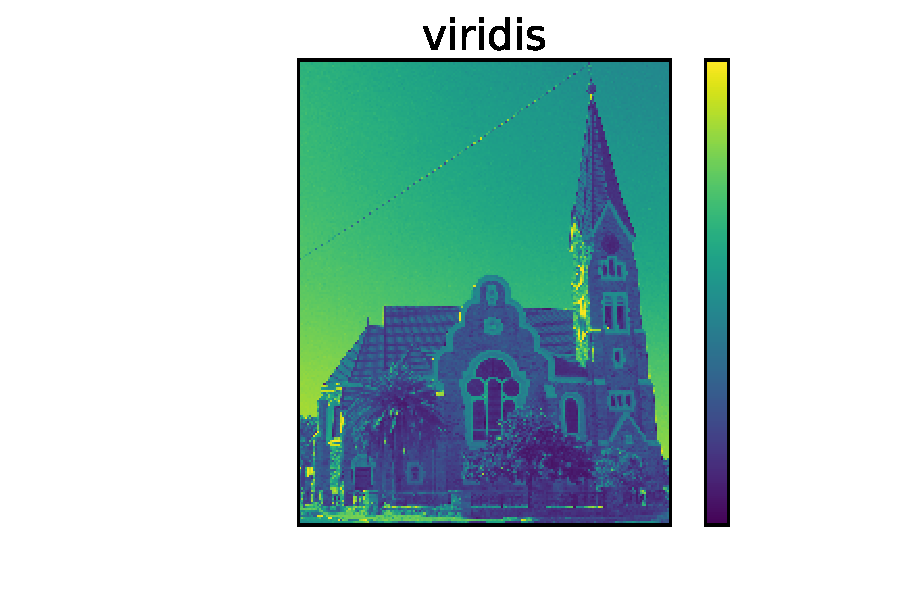
\includegraphics[width=0.42\textwidth]{../church_viridis.pdf}
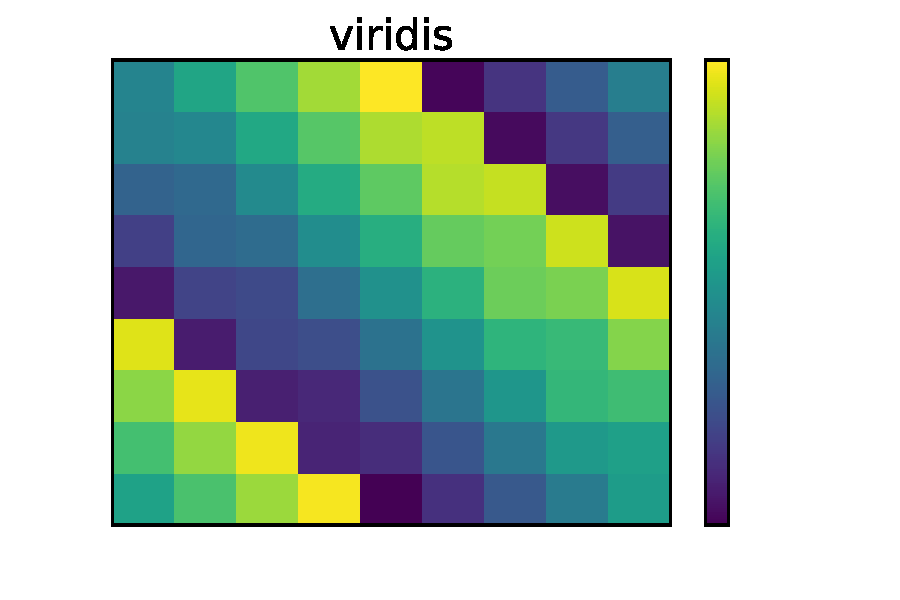
\includegraphics[width=0.58\textwidth]{../magicsquare_viridis.pdf}\newline\newline
\vfill
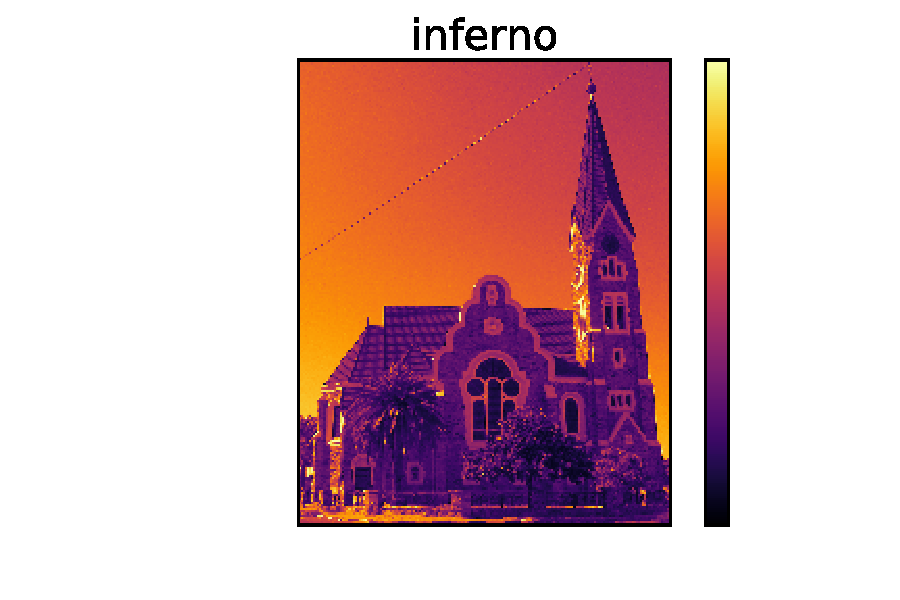
\includegraphics[width=0.42\textwidth]{../church_inferno.pdf}
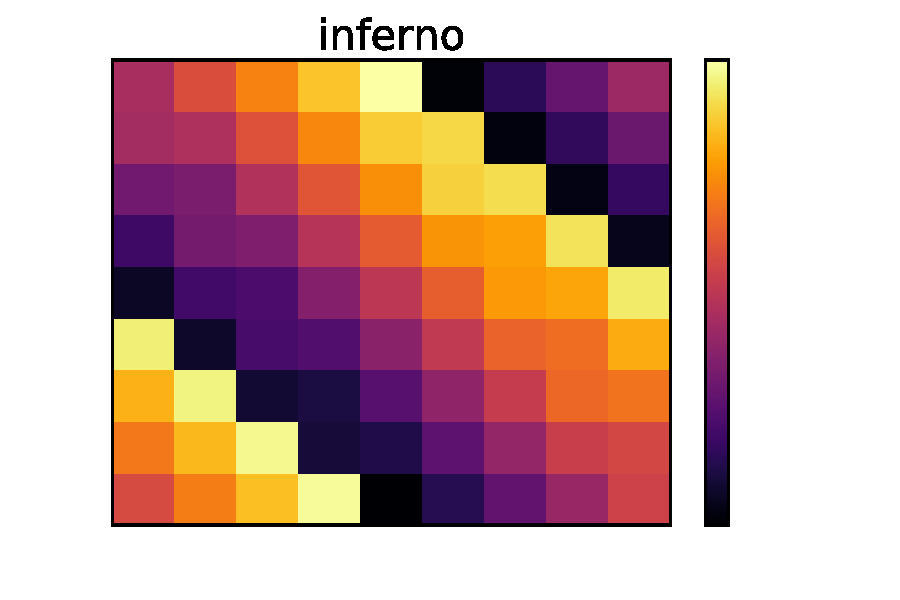
\includegraphics[width=0.58\textwidth]{../magicsquare_inferno.pdf}
\vfill
\end{center}
\end{column}
\end{columns}
\end{frame}

\begin{frame}[fragile]
\frametitle{Heatmaps with \texttt{pcolor}}
\vfill
\begin{center}
$f(x, y) = -\left(x^2+3y^2\right)e^{-x^2-y^2}$
\end{center}
\vfill
\tiny{
\begin{columns}
\begin{column}{0.35\textwidth}
\begin{minted}{python}
xs = np.arange(-2, 2.2, 0.1)
ys = np.arange(-2, 2.2, 0.1)

z = []
for y in ys[:-1]:
    z.append([])
    for x in xs[:-1]:
        z[-1].append(f(x, y))
\end{minted}
\end{column}
\begin{column}{0.65\textwidth}
\begin{equation*}
\begin{pmatrix}
-0.005 & -0.007 & -0.010 & \cdots & -0.010 & -0.007 & -0.005 \\
-0.008 & -0.011 & -0.014 & \cdots & -0.014 & -0.011 & -0.008 \\
-0.011 & -0.015 & -0.020 & \cdots & -0.020 & -0.015 & -0.011 \\
\vdots & \vdots & \vdots & \ddots & \vdots & \vdots & \vdots \\
-0.011 & -0.015 & -0.020 & \cdots & -0.020 & -0.015 & -0.011 \\
-0.008 & -0.011 & -0.014 & \cdots & -0.014 & -0.011 & -0.008 \\
-0.005 & -0.007 & -0.010 & \cdots & -0.010 & -0.007 & -0.005
\end{pmatrix}
\end{equation*}
\end{column}
\end{columns}
}
\vfill
\end{frame}


\begin{frame}[fragile]
\tiny{
\begin{columns}
\begin{column}{0.45\textwidth}
\begin{minted}{python}
fig, ax = plt.subplots(1)

hm = ax.pcolor(z)


















plt.show()
\end{minted}
\end{column}
\begin{column}{0.55\textwidth}
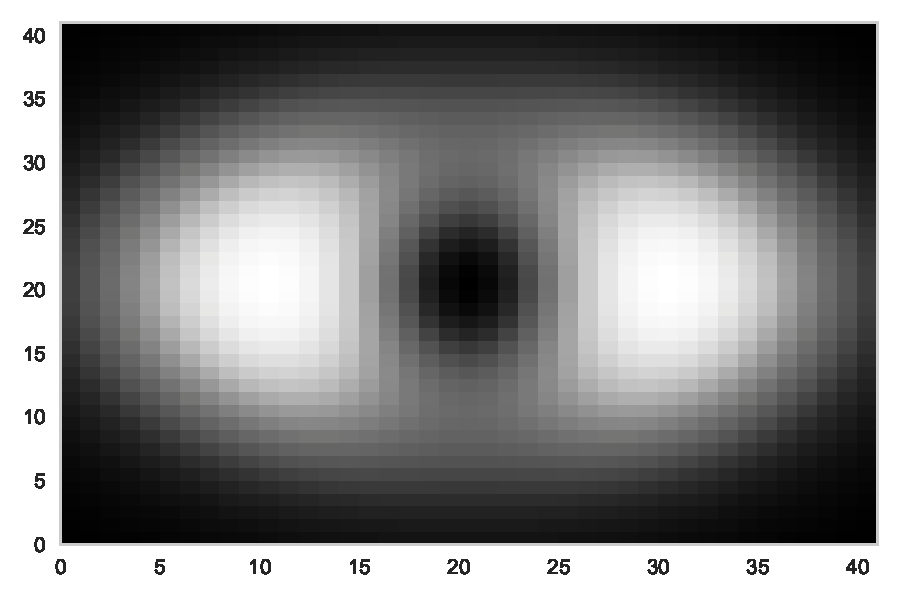
\includegraphics[width=\textwidth]{../heatmap_1.pdf}
\end{column}
\end{columns}
}
\end{frame}

\begin{frame}[fragile]
\tiny{
\begin{columns}
\begin{column}{0.45\textwidth}
\begin{minted}{python}
fig, ax = plt.subplots(1)
X,Y = np.meshgrid(xs, ys)
hm = ax.pcolor(X, Y, z)


















plt.show()
\end{minted}
\end{column}
\begin{column}{0.55\textwidth}
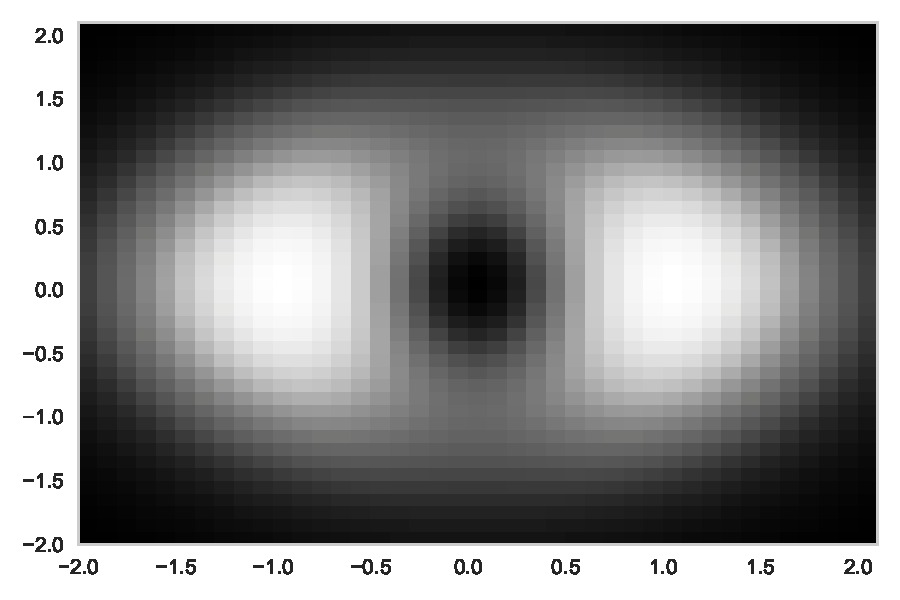
\includegraphics[width=\textwidth]{../heatmap_2.pdf}
\end{column}
\end{columns}
}
\end{frame}

\begin{frame}[fragile]
\tiny{
\begin{columns}
\begin{column}{0.45\textwidth}
\begin{minted}{python}
fig, ax = plt.subplots(1)
X,Y = np.meshgrid(xs, ys)
hm = ax.pcolor(X, Y, z, cmap='inferno')


















plt.show()
\end{minted}
\end{column}
\begin{column}{0.55\textwidth}
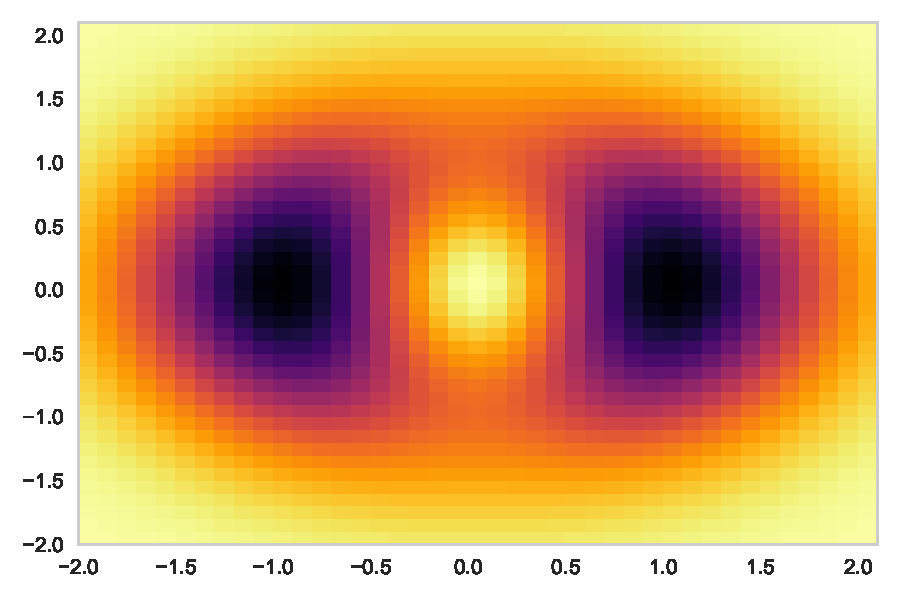
\includegraphics[width=\textwidth]{../heatmap_3.pdf}
\end{column}
\end{columns}
}
\end{frame}

\begin{frame}[fragile]
\tiny{
\begin{columns}
\begin{column}{0.45\textwidth}
\begin{minted}{python}
fig, ax = plt.subplots(1)
X,Y = np.meshgrid(xs, ys)
hm = ax.pcolor(X, Y, z, cmap='inferno')

ticks = np.linspace(-2, 2, 9)
ax.set_xticks([i+0.05 for i in ticks])
ax.set_yticks([i+0.05 for i in ticks])
ax.set_xticklabels(ticks)
ax.set_yticklabels(ticks)












plt.show()
\end{minted}
\end{column}
\begin{column}{0.55\textwidth}
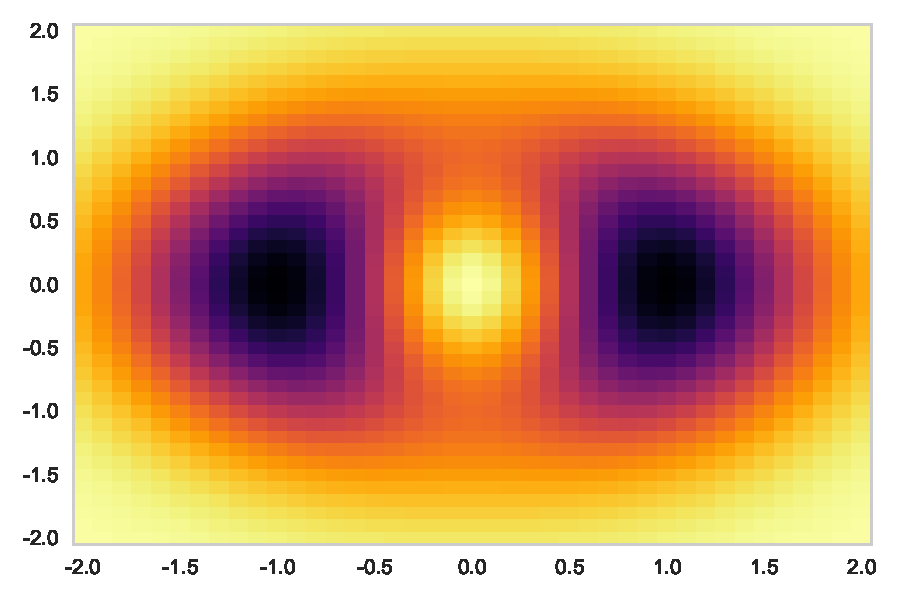
\includegraphics[width=\textwidth]{../heatmap_4.pdf}
\end{column}
\end{columns}
}
\end{frame}

\begin{frame}[fragile]
\tiny{
\begin{columns}
\begin{column}{0.45\textwidth}
\begin{minted}{python}
fig, ax = plt.subplots(1)
X,Y = np.meshgrid(xs, ys)
hm = ax.pcolor(X, Y, z, cmap='inferno')

ticks = np.linspace(-2, 2, 9)
ax.set_xticks([i+0.05 for i in ticks])
ax.set_yticks([i+0.05 for i in ticks])
ax.set_xticklabels(ticks)
ax.set_yticklabels(ticks)

cbar = fig.colorbar(hm)
cbar.set_label(r"$f(x, y)$")









plt.show()
\end{minted}
\end{column}
\begin{column}{0.55\textwidth}
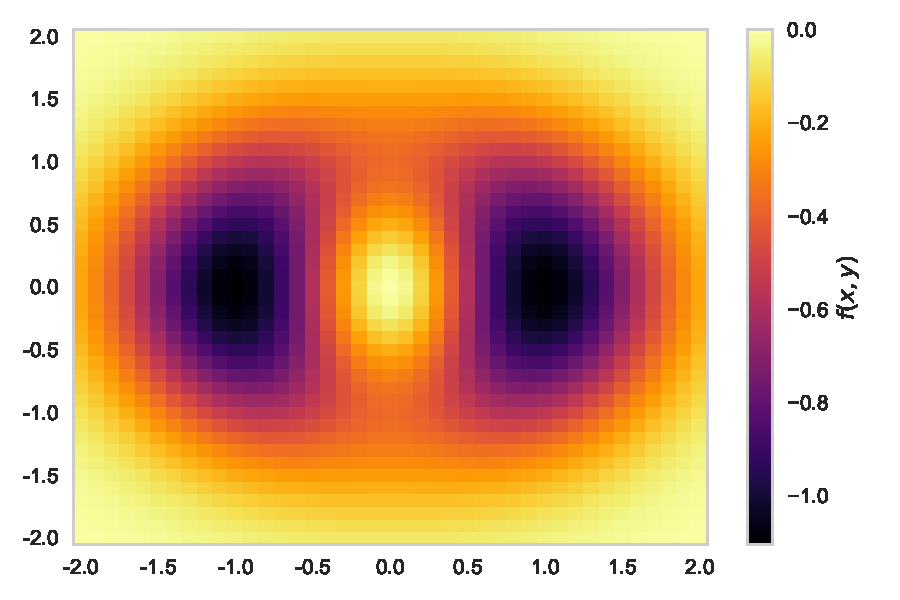
\includegraphics[width=\textwidth]{../heatmap_5.pdf}
\end{column}
\end{columns}
}
\end{frame}

\begin{frame}[fragile]
\tiny{
\begin{columns}
\begin{column}{0.45\textwidth}
\begin{minted}{python}
fig, ax = plt.subplots(1)
X,Y = np.meshgrid(xs, ys)
hm = ax.pcolor(X, Y, z, cmap='inferno')

ticks = np.linspace(-2, 2, 9)
ax.set_xticks([i+0.05 for i in ticks])
ax.set_yticks([i+0.05 for i in ticks])
ax.set_xticklabels(ticks)
ax.set_yticklabels(ticks)

cbar = fig.colorbar(hm)
cbar.set_label(r"$f(x, y)$")

title = r"$\left(x^2+3y^2\right)e^{-x^2-y^2}$"
ax.set_title(title, fontsize=18)
ax.set_xlabel(r"$x$", fontsize=16)
ax.set_ylabel(r"$y$", fontsize=16)




plt.show()
\end{minted}
\end{column}
\begin{column}{0.55\textwidth}
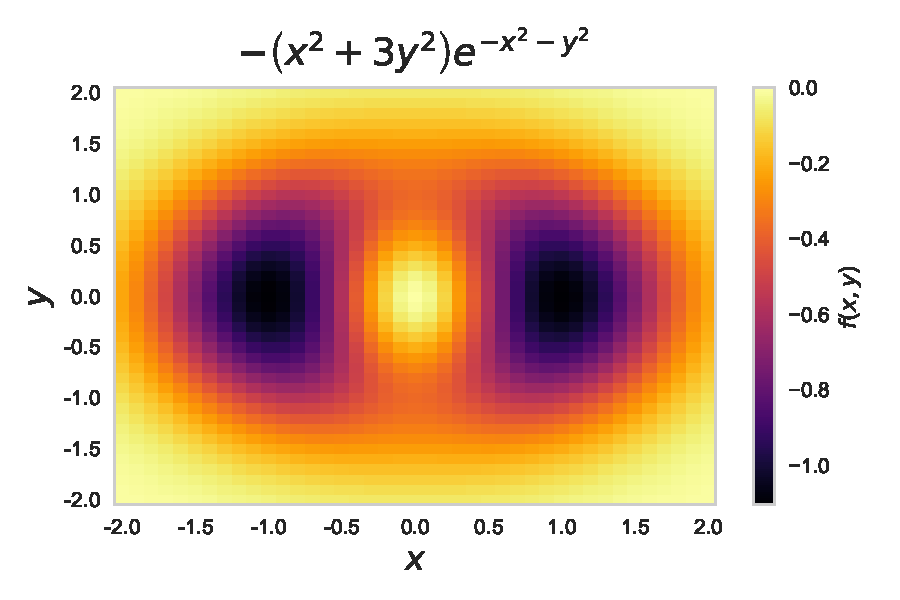
\includegraphics[width=\textwidth]{../heatmap_6.pdf}
\end{column}
\end{columns}
}
\end{frame}

\begin{frame}[fragile]
\tiny{
\begin{columns}
\begin{column}{0.45\textwidth}
\begin{minted}{python}
fig, ax = plt.subplots(1)
X,Y = np.meshgrid(xs, ys)
hm = ax.pcolor(X, Y, z, cmap='inferno', zorder=0)

ticks = np.linspace(-2, 2, 9)
ax.set_xticks([i+0.05 for i in ticks])
ax.set_yticks([i+0.05 for i in ticks])
ax.set_xticklabels(ticks)
ax.set_yticklabels(ticks)

cbar = fig.colorbar(hm)
cbar.set_label(r"$f(x, y)$")

title = r"$\left(x^2+3y^2\right)e^{-x^2-y^2}$"
ax.set_title(title, fontsize=18)
ax.set_xlabel(r"$x$", fontsize=16)
ax.set_ylabel(r"$y$", fontsize=16)

ax.grid(which='major', color='darkslategrey',
        linestyle=':', linewidth=1, axis='both')

plt.show()
\end{minted}
\end{column}
\begin{column}{0.55\textwidth}
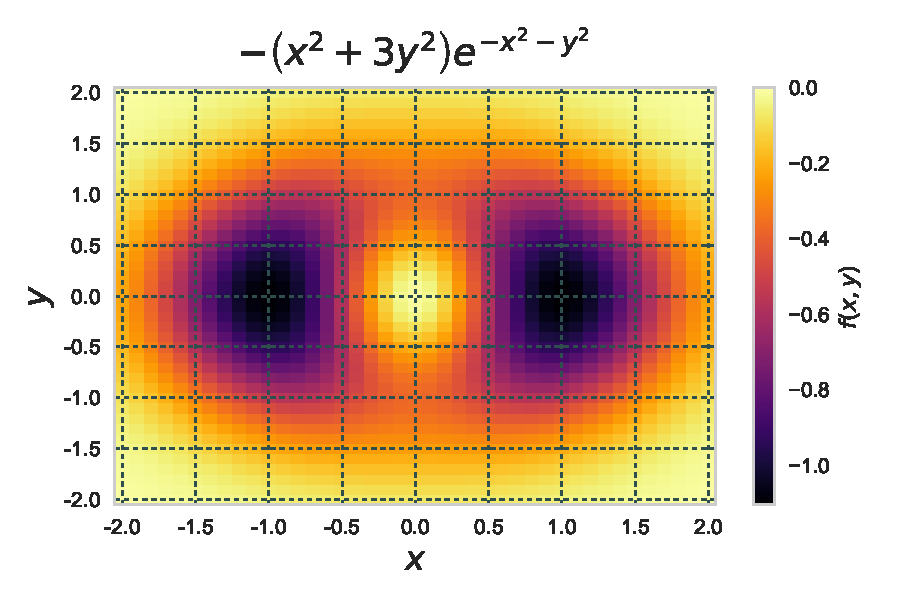
\includegraphics[width=\textwidth]{../heatmap_7.pdf}
\end{column}
\end{columns}
}
\end{frame}










\begin{frame}{{}}
\begin{center}
\includegraphics[width=0.21\textwidth]{cflogo}
\hspace{10mm}
\includegraphics[width=0.2\textwidth]{napycon_logo}
\vspace{5mm}
\begin{columns}
\begin{column}{0.7\textwidth}
\begin{itemize}
\item \href{http://www.cardiff.ac.uk/about/our-profile/our-values/engagement/transforming-communities/the-phoenix-project}{Cardiff University Phoenix Project}
\item \href{http://www.cardiff.ac.uk/mathematics}{Cardiff School of Mathematics}
\item \href{https://na.pycon.org/}{PyCon Namibia 2017}
\end{itemize}
\end{column}
\begin{column}{0.3\textwidth}
\begin{itemize}
\item \href{http://matplotlib.org/}{matplotlib}
\item \href{http://www.numpy.org/}{numpy}
\item \href{http://seaborn.pydata.org/}{seaborn}
\item \href{http://jupyter.org/}{jupyter}
\end{itemize}
\end{column}
\end{columns}
\vspace{5mm}
\textcolor{orange}{
\url{www.geraintianpalmer.org.uk/talks}\\
\href{https://twitter.com/GeraintPalmer}{@GeraintPalmer}
}
\end{center}
\end{frame}

\begin{frame}
\begin{center}
\huge{Links}
\end{center}
\scriptsize{
\begin{itemize}
\item \url{http://matplotlib.org/api/axes_api.html}
\item \url{http://matplotlib.org/api/pyplot_summary.html}
\item \url{http://matplotlib.org/examples/index.html}
\item \url{http://matplotlib.org/examples/color/colormaps_reference.html}
\item \url{https://www.youtube.com/watch?v=k_lvjRCOpJk&feature=youtu.be&list=PLpX1jXuNTXGrjl6CxJ6Cly1GKO1su9yeD}
\item \url{https://www.youtube.com/watch?v=k_lvjRCOpJk&feature=youtu.be&list=PLpX1jXuNTXGrjl6CxJ6Cly1GKO1su9yeD}
\item \url{https://vincentarelbundock.github.io/Rdatasets/datasets.html}
\item \url{http://www.databaseolympics.com/}
\item \url{https://en.wikipedia.org/wiki/Magic_square}
\end{itemize}
}
\end{frame}



\end{document}
